% !TEX program = pdflatex
% GDG on Campus JIS University — Technical Report 2022–
% GENERATED by build.py — edit data there, not here.
\documentclass[11pt,a4paper]{article}

\usepackage[T1]{fontenc}
\usepackage[utf8]{inputenc}
\usepackage[sfdefault]{roboto}
\usepackage[a4paper,top=2.4cm,bottom=2.2cm,left=2.0cm,right=2.0cm,headsep=14pt]{geometry}
\usepackage{graphicx}
\usepackage{xcolor}
\usepackage{tikz}
\usetikzlibrary{calc}
\usepackage[most]{tcolorbox}
\usepackage{fancyhdr}
\usepackage{fontawesome5}
\usepackage{enumitem}
\usepackage{tabularx}
\usepackage{array}
\usepackage{colortbl}
\usepackage{multicol}
\usepackage{csquotes}
\usepackage{needspace}
\usepackage[hidelinks]{hyperref}
\usepackage{bookmark}
\hypersetup{pdftitle={GDG on Campus JIS University — Technical Report 2022–},
            pdfauthor={Ayushman Bhattacharya},
            pdfsubject={Chapter technical report},
            bookmarksnumbered=false}

% ---- Google brand palette ----
\definecolor{GBlue}{HTML}{4285F4}
\definecolor{GRed}{HTML}{EA4335}
\definecolor{GYel}{HTML}{FBBC04}
\definecolor{GGrn}{HTML}{34A853}
\definecolor{Ink}{HTML}{202124}
\definecolor{Slate}{HTML}{5F6368}
\definecolor{Mist}{HTML}{F1F3F4}
\definecolor{Line}{HTML}{DADCE0}
\color{Ink}

% ---- running header / footer ----
\pagestyle{fancy}
\fancyhf{}
\renewcommand{\headrulewidth}{0pt}
\renewcommand{\footrulewidth}{0pt}
\fancyfoot[C]{\footnotesize\color{Slate}%
  \textcolor{GBlue}{\rule[-1pt]{7pt}{7pt}}\hspace{2pt}%
  GDG on Campus JIS University \,\textperiodcentered\, Technical Report \,\textperiodcentered\, Dept. of CSE}
\fancyfoot[R]{\footnotesize\color{Slate}\thepage}
\fancyhead[L]{\footnotesize\color{Slate}\leftmark}
\renewcommand{\sectionmark}[1]{\markboth{#1}{}}

\setlength{\parindent}{0pt}
\setlength{\parskip}{5pt}
\setlength{\emergencystretch}{1.5em}
% Event cards intentionally combine ragged title columns, rules and image
% grids; suppress harmless loose-box diagnostics while retaining overfull-box
% warnings, which indicate content escaping its allotted width.
\hbadness=10000

% four-colour rule used as a divider throughout
\newcommand{\gbar}[1][\linewidth]{%
  \begin{tikzpicture}
    \fill[GBlue] (0,0) rectangle (0.25*#1,0.11);
    \fill[GRed]  (0.25*#1,0) rectangle (0.50*#1,0.11);
    \fill[GYel]  (0.50*#1,0) rectangle (0.75*#1,0.11);
    \fill[GGrn]  (0.75*#1,0) rectangle (#1,0.11);
  \end{tikzpicture}}

% developer-brackets mark (vector), used as a small accent
\newcommand{\devmark}[1]{%
  \begin{tikzpicture}[x=1cm,y=1cm]
    \def\h{#1}
    \fill[GBlue] (0,0) -- (0.34*\h,0.5*\h) -- (0.12*\h,0.5*\h) -- (-0.22*\h,0) -- cycle;
    \fill[GRed]  (0,\h) -- (0.34*\h,0.5*\h) -- (0.12*\h,0.5*\h) -- (-0.22*\h,\h) -- cycle;
    \fill[GGrn]  (0.9*\h,0) -- (0.56*\h,0.5*\h) -- (0.78*\h,0.5*\h) -- (1.12*\h,0) -- cycle;
    \fill[GYel]  (0.9*\h,\h) -- (0.56*\h,0.5*\h) -- (0.78*\h,0.5*\h) -- (1.12*\h,\h) -- cycle;
  \end{tikzpicture}}

% framed image helper — width fills the column but height is capped so tall
% (portrait) photos can't overflow the page and push a gallery onto the next one.
\newlength{\galmaxh}\setlength{\galmaxh}{7.5cm}
\newcommand{\galimg}[1]{\setlength{\fboxsep}{0pt}\setlength{\fboxrule}{0.6pt}%
  \fcolorbox{Line}{white}{\includegraphics[
    width=\dimexpr\linewidth-2\fboxrule\relax,height=\galmaxh,keepaspectratio]{#1}}}

\begin{document}

% ============================== COVER ==============================
\thispagestyle{empty}
\vfill
\noindent\makebox[\linewidth][c]{
\includegraphics[width=\paperwidth]{assets/brand/banner_cover.png}}

\vspace{0.45cm}
\begin{center}
  
\includegraphics[width=2.3cm]{assets/brand/profile_dscjisu_native.png}\\[0.26cm]
  {\color{Slate}\large Department of Computer Science \& Engineering}\\[0.10cm]
  {\color{Slate}\normalsize JIS University, Kolkata}\\[0.7cm]

  {\fontsize{37}{41}\selectfont\bfseries\color{Ink} Technical Report}\\[0.26cm]
  {\Large\color{GBlue}\bfseries GDG on Campus \textperiodcentered\ JIS University}\\[0.34cm]
  {\large\color{Slate} Started in 2022 \,--}\\[0.55cm]
    \gbar[9cm]\\[0.55cm]
    {\small\itshape\color{Slate}``what a privilege it is\\
    to be exhausted by an ambition\\
    of your own choosing''}\\[0.75cm]
\end{center}
\vfill
\clearpage


% ============================== FOREWORD ==============================
\phantomsection\addcontentsline{toc}{section}{Foreword \& About this Report}
\section*{\color{Ink}Foreword \& About this Report}
\gbar[\linewidth]\\[10pt]

\textbf{GDG on Campus JIS University} — formerly \emph{Google Developer Student Clubs (GDSC)} —
is a student-led technical community operating under the Department of Computer Science \&
Engineering, JIS University. Run \emph{by the students, for the students}, it has grown across
four operational years into one of the largest and most active student organisations in the
university, with a community of \textbf{$\sim$1{,}800 members} drawn from every academic
background.

We build across Artificial Intelligence, Web Development, Cloud Computing, Cybersecurity, Mobile
Development, Open Source and System Design — through workshops, hackathons, bootcamps, speaker
sessions and study jams. Beyond the technical, we invest in peer mentorship, teamwork and
community-driven growth, so that each cohort leaves stronger than it arrived and sets the bar for
the next.

\vspace{4pt}
\begin{tcolorbox}[enhanced,colback=Mist,colframe=Mist,arc=4pt,left=14pt,right=14pt,top=10pt,bottom=10pt,
    borderline west={3pt}{0pt}{GBlue}]
  {\bfseries\color{Ink}Why this document exists.}\\[2pt]
  This is the chapter's institutional memory. Leadership turns over every year; the work should not
  start from zero each time. The report records \emph{what was run, by whom, with which partners, and
  at what scale} — season by season, since 2022. It is deliberately factual: event totals are
  reported as recorded, and event details are preserved as documented by the organising
  team of each season.
\end{tcolorbox}

\begin{tcolorbox}[enhanced,colback=white,colframe=GGrn,boxrule=1pt,arc=4pt,
    left=14pt,right=14pt,top=10pt,bottom=10pt]
  {\bfseries\color{GGrn}\faArrowRight~For the next lead.}\\[2pt]
  A community is only as strong as the memory it keeps. You inherit not just a chapter, but a
  promise — that the people who came before you are not forgotten, and that the people who come
  after you will stand on something solid. Add your season honestly, in full, and in your own voice.
  Nothing here belongs to any one of us; it belongs to whoever chooses to carry it next. When your
  time is done, hand it forward — a little larger, a little truer than you found it.
\end{tcolorbox}

\vspace{6pt}
{\footnotesize\color{Slate}\textbf{A note on numbering \& naming.} The original working records
carried a few clerical artefacts (a skipped index, a split entry, and the mid-life rebrand from
GDSC to GDG). This report renumbers all events sequentially and notes the brand in force each
season; no events were added or removed in doing so.}
\clearpage


% ============================== AT A GLANCE ==============================
\phantomsection\addcontentsline{toc}{section}{At a Glance (2022–26)}
\section*{\color{Ink}At a Glance \normalsize\color{Slate}(2022–26)}
\gbar[\linewidth]\\[8pt]
\noindent\begin{minipage}[t]{0.245\linewidth}\begin{tcolorbox}[enhanced,colback=white,colframe=Line,boxrule=0.6pt,arc=5pt,width=\linewidth,left=10pt,right=10pt,top=9pt,bottom=9pt,borderline north={3pt}{0pt}{GBlue}]{\color{GBlue}\large\faIcon{calendar-check}}\quad{\fontsize{25}{25}\selectfont\bfseries\color{Ink}4}\\[1pt]{\footnotesize\color{Slate}Seasons on record}\end{tcolorbox}\end{minipage}\hfill\begin{minipage}[t]{0.245\linewidth}\begin{tcolorbox}[enhanced,colback=white,colframe=Line,boxrule=0.6pt,arc=5pt,width=\linewidth,left=10pt,right=10pt,top=9pt,bottom=9pt,borderline north={3pt}{0pt}{GRed}]{\color{GRed}\large\faIcon{layer-group}}\quad{\fontsize{25}{25}\selectfont\bfseries\color{Ink}37}\\[1pt]{\footnotesize\color{Slate}Events held}\end{tcolorbox}\end{minipage}\hfill\begin{minipage}[t]{0.245\linewidth}\begin{tcolorbox}[enhanced,colback=white,colframe=Line,boxrule=0.6pt,arc=5pt,width=\linewidth,left=10pt,right=10pt,top=9pt,bottom=9pt,borderline north={3pt}{0pt}{GYel}]{\color{GYel}\large\faIcon{users}}\quad{\fontsize{25}{25}\selectfont\bfseries\color{Ink}4.4{\small k}}\\[1pt]{\footnotesize\color{Slate}Cumulative footfall}\end{tcolorbox}\end{minipage}\hfill\begin{minipage}[t]{0.245\linewidth}\begin{tcolorbox}[enhanced,colback=white,colframe=Line,boxrule=0.6pt,arc=5pt,width=\linewidth,left=10pt,right=10pt,top=9pt,bottom=9pt,borderline north={3pt}{0pt}{GGrn}]{\color{GGrn}\large\faIcon{user-friends}}\quad{\fontsize{25}{25}\selectfont\bfseries\color{Ink}\textasciitilde\,1.8{\small k}}\\[1pt]{\footnotesize\color{Slate}Community members}\end{tcolorbox}\end{minipage}
\vspace{9pt}

{\bfseries\color{Ink}Events per season}\quad{\footnotesize\color{Slate}— cadence has grown every year, from 3 in the founding season to 22 in 2025–26.}
\begin{center}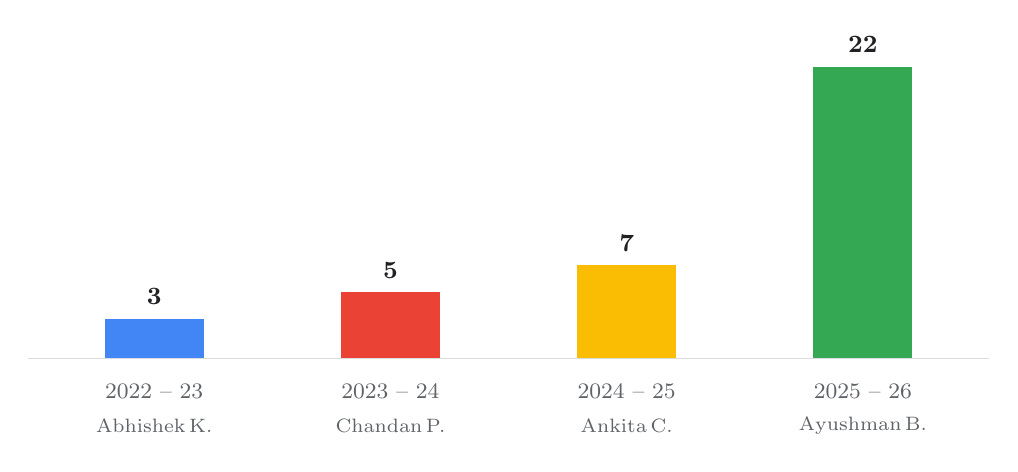
\begin{tikzpicture}[x=1cm,y=1cm]\draw[Line] (-0.1,0) -- (12.10,0);\fill[GBlue] (0.87,0) rectangle (2.13,0.50);\node[font=\bfseries\small,color=Ink] at (1.50,0.78) {3};\fill[GRed] (3.87,0) rectangle (5.13,0.84);\node[font=\bfseries\small,color=Ink] at (4.50,1.12) {5};\fill[GYel] (6.87,0) rectangle (8.13,1.18);\node[font=\bfseries\small,color=Ink] at (7.50,1.46) {7};\fill[GGrn] (9.87,0) rectangle (11.13,3.70);\node[font=\bfseries\small,color=Ink] at (10.50,3.98) {22};\node[font=\footnotesize,color=Slate,align=center] at (1.50,-0.42) {2022 – 23};\node[font=\scriptsize,color=Slate,align=center] at (1.50,-0.86) {Abhishek\,K.};\node[font=\footnotesize,color=Slate,align=center] at (4.50,-0.42) {2023 – 24};\node[font=\scriptsize,color=Slate,align=center] at (4.50,-0.86) {Chandan\,P.};\node[font=\footnotesize,color=Slate,align=center] at (7.50,-0.42) {2024 – 25};\node[font=\scriptsize,color=Slate,align=center] at (7.50,-0.86) {Ankita\,C.};\node[font=\footnotesize,color=Slate,align=center] at (10.50,-0.42) {2025 – 26};\node[font=\scriptsize,color=Slate,align=center] at (10.50,-0.86) {Ayushman\,B.};\end{tikzpicture}\end{center}
\vspace{8pt}

{\bfseries\color{Ink}Community growth}\quad{\footnotesize\color{Slate}— approximate registered membership at the close of each season, from a founding cohort of well under a hundred to around 1,800 today.}
\begin{center}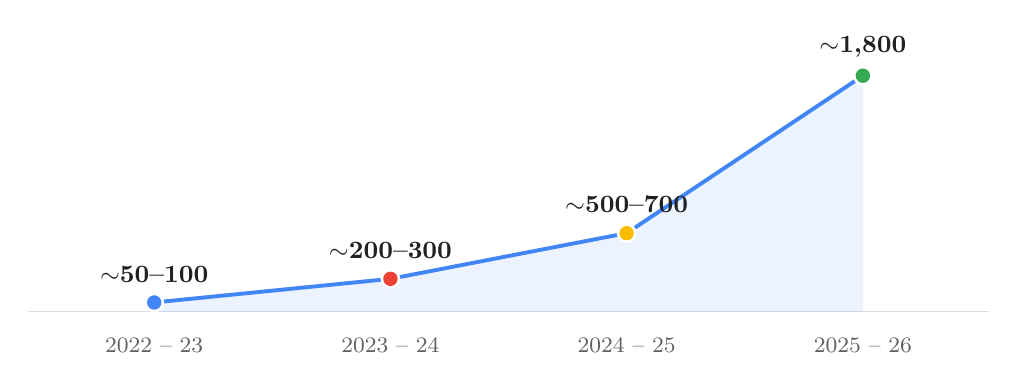
\begin{tikzpicture}[x=1cm,y=1cm]\draw[Line] (-0.1,0) -- (12.10,0);\fill[GBlue,opacity=0.10] (1.50,0) -- (1.50,0.12) -- (4.50,0.42) -- (7.50,1.00) -- (10.50,3.00) -- (10.50,0) -- cycle;\draw[GBlue,line width=1.4pt] (1.50,0.12) -- (4.50,0.42) -- (7.50,1.00) -- (10.50,3.00);\fill[white] (1.50,0.12) circle (3.6pt);\fill[GBlue] (1.50,0.12) circle (2.6pt);\fill[white] (4.50,0.42) circle (3.6pt);\fill[GRed] (4.50,0.42) circle (2.6pt);\fill[white] (7.50,1.00) circle (3.6pt);\fill[GYel] (7.50,1.00) circle (2.6pt);\fill[white] (10.50,3.00) circle (3.6pt);\fill[GGrn] (10.50,3.00) circle (2.6pt);\node[font=\bfseries\small,color=Ink] at (1.50,0.48) {$\sim$50–100};\node[font=\footnotesize,color=Slate] at (1.50,-0.42) {2022 – 23};\node[font=\bfseries\small,color=Ink] at (4.50,0.78) {$\sim$200–300};\node[font=\footnotesize,color=Slate] at (4.50,-0.42) {2023 – 24};\node[font=\bfseries\small,color=Ink] at (7.50,1.36) {$\sim$500–700};\node[font=\footnotesize,color=Slate] at (7.50,-0.42) {2024 – 25};\node[font=\bfseries\small,color=Ink] at (10.50,3.36) {$\sim$1,800};\node[font=\footnotesize,color=Slate] at (10.50,-0.42) {2025 – 26};\end{tikzpicture}\end{center}
\vspace{6pt}
\renewcommand{\arraystretch}{1.15}\begin{tabularx}{\linewidth}{@{}l l X c r r r@{}}\multicolumn{7}{@{}l}{\footnotesize\color{Slate}\textsc{Season ledger}}\\[3pt]\textbf{Season} & \textbf{Brand} & \textbf{Organiser} & \textbf{Core} & \textbf{Members} & \textbf{Events} & \textbf{Footfall}\\\arrayrulecolor{Line}\hline\rule{0pt}{1ex}\rule{0pt}{2.6ex}\textcolor{GBlue}{\rule[-0.2ex]{8pt}{8pt}}~\textbf{2022 – 23} & GDSC & Abhishek Kushwaha & 5 & $\sim$50–100 & 3 & 315 \\[2pt]\rule{0pt}{2.6ex}\textcolor{GRed}{\rule[-0.2ex]{8pt}{8pt}}~\textbf{2023 – 24} & GDSC & Chandan Pandey & 6 & $\sim$200–300 & 5 & 425 \\[2pt]\rule{0pt}{2.6ex}\textcolor{GYel}{\rule[-0.2ex]{8pt}{8pt}}~\textbf{2024 – 25} & GDG & Ankita Chakraborty & 8 & $\sim$500–700 & 7 & 565 \\[2pt]\rule{0pt}{2.6ex}\textcolor{GGrn}{\rule[-0.2ex]{8pt}{8pt}}~\textbf{2025 – 26} & GDG & Ayushman Bhattacharya & 17 & $\sim$1,800 & 22 & 3,139 \\[2pt]\hline\rule{0pt}{2.4ex}\textbf{Total} & & & & \textbf{$\sim$1,800} & \textbf{37} & \textbf{4,444}\\\end{tabularx}

\vspace{8pt}
{\footnotesize\color{Slate}\emph{Footfall} is cumulative event participation across the season (range
midpoints where a range was recorded); attendees recur across events, so this counts participation,
not unique members.}
\clearpage


% ============================== LINEAGE ==============================
\phantomsection\addcontentsline{toc}{section}{Leadership Lineage (2022–26)}
\section*{\color{Ink}Leadership Lineage \normalsize\color{Slate}(2022–26)}
\gbar[\linewidth]\\[10pt]
{\color{Slate}Each organiser inherited a chapter and grew it, from 2022 to 2026. This is the chain of custody.}
\vspace{12pt}
\begin{itemize}[leftmargin=1.8em,itemsep=22pt,parsep=0pt,label=\textcolor{GBlue}{\faCircle}]
\item[\textcolor{GBlue}{\faCircle}] {\large\textbf{2022 – 23}}\;\textcolor{Slate}{\small(GDSC)}\\[3pt]\textbf{Abhishek Kushwaha} \;{\color{Slate}— Founding Organiser}\\[3pt]{\small\color{Slate}Roll No.~}\rule[-2pt]{3.4cm}{0.4pt}\\[5pt]{\small\color{Slate}The founding season. The chapter is established under the Department of Computer Science \& Engineering and runs its first info session, its first external speaker workshop, and its first hosted codefest.}
\item[\textcolor{GRed}{\faCircle}] {\large\textbf{2023 – 24}}\;\textcolor{Slate}{\small(GDSC)}\\[3pt]\textbf{Chandan Pandey} \;{\color{Slate}— Organiser}\\[3pt]{\small\color{Slate}Roll No.~}\rule[-2pt]{3.4cm}{0.4pt}\\[5pt]{\small\color{Slate}Consolidation. Study Jams and a source-code contribution drive push the chapter deeper into cloud skilling and open source, alongside the annual onboarding session and a hands-on web bootcamp.}
\item[\textcolor{GYel}{\faCircle}] {\large\textbf{2024 – 25}}\;\textcolor{Slate}{\small(GDG)}\\[3pt]\textbf{Ankita Chakraborty} \;{\color{Slate}— Organiser}\\[3pt]{\small\color{Slate}Roll No.~}\rule[-2pt]{3.4cm}{0.4pt}\\[5pt]{\small\color{Slate}Rebrand to Google Developer Groups (GDG) on Campus and a step-up in cadence: cross-chapter collaborations (Solution Challenge, React), security and Web3 tracks, and the first Build with AI.}
\item[\textcolor{GGrn}{\faCircle}] {\large\textbf{2025 – 26}}\;\textcolor{Slate}{\small(GDG)}\\[3pt]\textbf{Ayushman Bhattacharya} \;{\color{Slate}— Organiser (current)}\\[3pt]{\small\color{Slate}Roll No.~}\textbf{23CS2021016}\\[5pt]{\small\color{Slate}The largest season on record — national hackathons, Hacktoberfest, GSoC preparation, live CTF and system-design tracks, a Kubernetes/CNCF meetup and cross-community welcomes with OWASP. This report is compiled during, and as part of, this tenure.}
\end{itemize}
\clearpage


\phantomsection\addcontentsline{toc}{section}{Contents (2022–26)}
\section*{\color{Ink}Contents \normalsize\color{Slate}(2022–26)}
\gbar[\linewidth]\\[8pt]
\begingroup
\hypersetup{linkcolor=Ink}
\renewcommand{\contentsname}{}
\vspace{-3.4em}
\tableofcontents
\endgroup
\clearpage


\clearpage
\phantomsection
\addcontentsline{toc}{section}{Season 2022 – 23 \textbullet\ Abhishek Kushwaha}
\markboth{Season 2022 – 23}{}
\begin{tcolorbox}[enhanced,colback=GBlue,colframe=GBlue,arc=6pt,
    left=18pt,right=18pt,top=12pt,bottom=12pt,fontupper=\color{white}]
  {\LARGE\bfseries 2022 – 23}\hfill{\normalsize\itshape Google Developer Student Clubs}\\[6pt]
  {\large Organiser \;\textbf{Abhishek Kushwaha}}\\[8pt]
  {\small The founding season. The chapter is established under the Department of Computer Science \& Engineering and runs its first info session, its first external speaker workshop, and its first hosted codefest.}\\[10pt]
  \textcolor{white}{\rule{\linewidth}{0.6pt}}\\[6pt]
  {\small\mbox{\faLayerGroup~\textbf{3} events} \quad\mbox{\faUserFriends~\textbf{5} core} \quad\mbox{\faUserPlus~\textbf{$\sim$50–100} members} \quad\mbox{\faUsers~\textbf{315} footfall} \quad\mbox{\faTag~GDSC brand}}
\end{tcolorbox}
\vspace{5pt}

\Needspace{7cm}
\phantomsection\addcontentsline{toc}{subsection}{01.~Info Session — Class of 2022–23}
\begin{tcolorbox}[enhanced,breakable,colback=white,colframe=Line,boxrule=0.6pt,arc=5pt,
    left=14pt,right=14pt,top=12pt,bottom=12pt,
    borderline west={3.5pt}{0pt}{GBlue},before skip=8pt,after skip=12pt]
  \noindent\begin{tabularx}{\linewidth}{@{}c@{\hspace{7pt}}>{\raggedright\arraybackslash}X@{\hspace{7pt}}r@{}}
    \tikz[baseline]{\node[fill=GBlue,text=white,font=\bfseries\small,rounded corners=3pt,inner xsep=6pt,inner ysep=2.5pt] {01};} & {\large\bfseries\color{Ink}Info Session — Class of 2022–23} & \tikz[baseline]{\node[fill=GGrn,text=white,font=\footnotesize\bfseries,rounded corners=3pt,inner xsep=6pt,inner ysep=2.5pt] {\faIcon{map-marker-alt}~On-Site};}
  \end{tabularx}\\[8pt]
  {\color{Line}\rule{\linewidth}{0.5pt}}\\[7pt]
  {\small\color{Ink!85}The founding season's opening event. It introduced GDSC JIS University to a fresh cohort — the community's mission, the technical domains it would explore, and the ways students could take part as members and volunteers. As the first gathering under the newly-formed chapter, it doubled as the recruitment drive for the founding core team.}\\[9pt]\renewcommand{\arraystretch}{1.05}\begin{tabularx}{\linewidth}{@{}c l X@{}}\textcolor{Slate}{\faIcon{calendar-alt}} & \textbf{Date} & 27 August 2022\,\textperiodcentered\,JIS University \\[3pt]\textcolor{Slate}{\faIcon{clock}} & \textbf{Duration} & 11:00 AM IST \\[3pt]\textcolor{Slate}{\faIcon{microphone}} & \textbf{Speaker(s)} & Abhishek Kushwaha \\[3pt]\textcolor{Slate}{\faIcon{handshake}} & \textbf{Partners} & — \\[3pt]\textcolor{Slate}{\faIcon{users}} & \textbf{Participation} & \textbf{90} participants \\[3pt]\end{tabularx}
  \vspace{4pt}
  \Needspace{4cm}\vspace{9pt}\noindent{\color{Line}\rule{\linewidth}{0.7pt}}\\[4pt]{\footnotesize\bfseries\color{Slate}\faImages~~EVENT GALLERY}\hfill\raisebox{1pt}{\gbar[4.2cm]}\\[7pt]\noindent \begin{minipage}[t]{0.485\linewidth}\centering \galimg{assets/gallery/01/img-01.jpg} \end{minipage}\hfill\begin{minipage}[t]{0.485\linewidth}\centering \galimg{assets/gallery/01/img-02.jpg} \end{minipage}
\end{tcolorbox}

\vspace{1pt}\centerline{\gbar[6cm]}\vspace{6pt}
\Needspace{7cm}
\phantomsection\addcontentsline{toc}{subsection}{02.~Interacting with the Unique Blockchain: From Zero to Hero}
\begin{tcolorbox}[enhanced,breakable,colback=white,colframe=Line,boxrule=0.6pt,arc=5pt,
    left=14pt,right=14pt,top=12pt,bottom=12pt,
    borderline west={3.5pt}{0pt}{GRed},before skip=8pt,after skip=12pt]
  \noindent\begin{tabularx}{\linewidth}{@{}c@{\hspace{7pt}}>{\raggedright\arraybackslash}X@{\hspace{7pt}}r@{}}
    \tikz[baseline]{\node[fill=GRed,text=white,font=\bfseries\small,rounded corners=3pt,inner xsep=6pt,inner ysep=2.5pt] {02};} & {\large\bfseries\color{Ink}Interacting with the Unique Blockchain: From Zero to Hero} & \tikz[baseline]{\node[fill=GBlue,text=white,font=\footnotesize\bfseries,rounded corners=3pt,inner xsep=6pt,inner ysep=2.5pt] {\faIcon{wifi}~Virtual};}
  \end{tabularx}\\[8pt]
  {\color{Line}\rule{\linewidth}{0.5pt}}\\[7pt]
  {\small\color{Ink!85}A beginner-friendly virtual workshop on the Unique Network / Polkadot ecosystem, delivered by an industry developer. It walked students with no prior Web3 background through the fundamentals of building on a substrate-based blockchain, and broadened the chapter's early programming beyond web and cloud into emerging decentralised technology.}\\[9pt]\renewcommand{\arraystretch}{1.05}\begin{tabularx}{\linewidth}{@{}c l X@{}}\textcolor{Slate}{\faIcon{calendar-alt}} & \textbf{Date} & 3 September 2022\,\textperiodcentered\,JIS University \\[3pt]\textcolor{Slate}{\faIcon{clock}} & \textbf{Duration} & 4:00 PM IST \\[3pt]\textcolor{Slate}{\faIcon{microphone}} & \textbf{Speaker(s)} & Alexander Saft \\[3pt]\textcolor{Slate}{\faIcon{handshake}} & \textbf{Partners} & Unique \\[3pt]\textcolor{Slate}{\faIcon{users}} & \textbf{Participation} & \textbf{70–80} participants \\[3pt]\end{tabularx}
  \vspace{4pt}
  \Needspace{4cm}\vspace{9pt}\noindent{\color{Line}\rule{\linewidth}{0.7pt}}\\[4pt]{\footnotesize\bfseries\color{Slate}\faImages~~EVENT GALLERY}\hfill\raisebox{1pt}{\gbar[4.2cm]}\\[7pt]\begin{center}\begin{minipage}{0.62\linewidth}\galimg{assets/gallery/02/img-01.jpg}\end{minipage}\end{center}
\end{tcolorbox}

\vspace{1pt}\centerline{\gbar[6cm]}\vspace{6pt}
\Needspace{7cm}
\phantomsection\addcontentsline{toc}{subsection}{03.~GDG JISU Codefest 2023}
\begin{tcolorbox}[enhanced,breakable,colback=white,colframe=Line,boxrule=0.6pt,arc=5pt,
    left=14pt,right=14pt,top=12pt,bottom=12pt,
    borderline west={3.5pt}{0pt}{GYel},before skip=8pt,after skip=12pt]
  \noindent\begin{tabularx}{\linewidth}{@{}c@{\hspace{7pt}}>{\raggedright\arraybackslash}X@{\hspace{7pt}}r@{}}
    \tikz[baseline]{\node[fill=GYel,text=white,font=\bfseries\small,rounded corners=3pt,inner xsep=6pt,inner ysep=2.5pt] {03};} & {\large\bfseries\color{Ink}GDG JISU Codefest 2023} & \tikz[baseline]{\node[fill=GGrn,text=white,font=\footnotesize\bfseries,rounded corners=3pt,inner xsep=6pt,inner ysep=2.5pt] {\faIcon{map-marker-alt}~On-Site};}
  \end{tabularx}\\[8pt]
  {\color{Line}\rule{\linewidth}{0.5pt}}\\[7pt]
  {\small\color{Ink!85}The chapter's first hosted competitive-coding event, run on-site across a full day. Spanning tooling from GitHub, Flutter, Firebase and Android, it put 150 students in a deadline-driven build environment with mentors on the floor. Codefest established the chapter's flagship habit of large, practical, project-first gatherings.}\\[9pt]\renewcommand{\arraystretch}{1.05}\begin{tabularx}{\linewidth}{@{}c l X@{}}\textcolor{Slate}{\faIcon{calendar-alt}} & \textbf{Date} & 21 March 2023\,\textperiodcentered\,JIS University \\[3pt]\textcolor{Slate}{\faIcon{clock}} & \textbf{Duration} & 10:00 AM – 3:30 PM \\[3pt]\textcolor{Slate}{\faIcon{microphone}} & \textbf{Speaker(s)} & Arkaprabha Chakraborty, Manish Kr Barnwal, Soumyadeep Chowdhury, Shubhayu Majumder \\[3pt]\textcolor{Slate}{\faIcon{handshake}} & \textbf{Partners} & GitHub, Flutter, Firebase, Android \\[3pt]\textcolor{Slate}{\faIcon{users}} & \textbf{Participation} & \textbf{150} participants \\[3pt]\end{tabularx}
  \vspace{4pt}
  \Needspace{4cm}\vspace{9pt}\noindent{\color{Line}\rule{\linewidth}{0.7pt}}\\[4pt]{\footnotesize\bfseries\color{Slate}\faImages~~EVENT GALLERY}\hfill\raisebox{1pt}{\gbar[4.2cm]}\\[7pt]\noindent \begin{minipage}[t]{0.485\linewidth}\centering \galimg{assets/gallery/03/img-01.jpg} \end{minipage}\hfill\begin{minipage}[t]{0.485\linewidth}\centering \galimg{assets/gallery/03/img-02.jpg} \end{minipage}
\end{tcolorbox}

\vspace{1pt}\centerline{\gbar[6cm]}\vspace{6pt}

\clearpage
\phantomsection
\addcontentsline{toc}{section}{Season 2023 – 24 \textbullet\ Chandan Pandey}
\markboth{Season 2023 – 24}{}
\begin{tcolorbox}[enhanced,colback=GRed,colframe=GRed,arc=6pt,
    left=18pt,right=18pt,top=12pt,bottom=12pt,fontupper=\color{white}]
  {\LARGE\bfseries 2023 – 24}\hfill{\normalsize\itshape Google Developer Student Clubs}\\[6pt]
  {\large Organiser \;\textbf{Chandan Pandey}}\\[8pt]
  {\small Consolidation. Study Jams and a source-code contribution drive push the chapter deeper into cloud skilling and open source, alongside the annual onboarding session and a hands-on web bootcamp.}\\[10pt]
  \textcolor{white}{\rule{\linewidth}{0.6pt}}\\[6pt]
  {\small\mbox{\faLayerGroup~\textbf{5} events} \quad\mbox{\faUserFriends~\textbf{6} core} \quad\mbox{\faUserPlus~\textbf{$\sim$200–300} members} \quad\mbox{\faUsers~\textbf{425} footfall} \quad\mbox{\faTag~GDSC brand}}
\end{tcolorbox}
\vspace{5pt}

\Needspace{7cm}
\phantomsection\addcontentsline{toc}{subsection}{04.~Info Session — Class of 2023–24}
\begin{tcolorbox}[enhanced,breakable,colback=white,colframe=Line,boxrule=0.6pt,arc=5pt,
    left=14pt,right=14pt,top=12pt,bottom=12pt,
    borderline west={3.5pt}{0pt}{GGrn},before skip=8pt,after skip=12pt]
  \noindent\begin{tabularx}{\linewidth}{@{}c@{\hspace{7pt}}>{\raggedright\arraybackslash}X@{\hspace{7pt}}r@{}}
    \tikz[baseline]{\node[fill=GGrn,text=white,font=\bfseries\small,rounded corners=3pt,inner xsep=6pt,inner ysep=2.5pt] {04};} & {\large\bfseries\color{Ink}Info Session — Class of 2023–24} & \tikz[baseline]{\node[fill=GGrn,text=white,font=\footnotesize\bfseries,rounded corners=3pt,inner xsep=6pt,inner ysep=2.5pt] {\faIcon{map-marker-alt}~On-Site};}
  \end{tabularx}\\[8pt]
  {\color{Line}\rule{\linewidth}{0.5pt}}\\[7pt]
  {\small\color{Ink!85}The annual onboarding session opening the 2023–24 cycle under new leadership. It re-introduced the community to incoming students and re-recruited the year's volunteer core, framing the roadmap of workshops, study jams and hackathons to come.}\\[9pt]\renewcommand{\arraystretch}{1.05}\begin{tabularx}{\linewidth}{@{}c l X@{}}\textcolor{Slate}{\faIcon{calendar-alt}} & \textbf{Date} & 19 September 2023\,\textperiodcentered\,JIS University \\[3pt]\textcolor{Slate}{\faIcon{clock}} & \textbf{Duration} & 11:00 AM IST \\[3pt]\textcolor{Slate}{\faIcon{microphone}} & \textbf{Speaker(s)} & Chandan Pandey \\[3pt]\textcolor{Slate}{\faIcon{handshake}} & \textbf{Partners} & — \\[3pt]\textcolor{Slate}{\faIcon{users}} & \textbf{Participation} & \textbf{120} participants \\[3pt]\end{tabularx}
  \vspace{4pt}
  \Needspace{4cm}\vspace{9pt}\noindent{\color{Line}\rule{\linewidth}{0.7pt}}\\[4pt]{\footnotesize\bfseries\color{Slate}\faImages~~EVENT GALLERY}\hfill\raisebox{1pt}{\gbar[4.2cm]}\\[7pt]\noindent \begin{minipage}[t]{0.485\linewidth}\centering \galimg{assets/gallery/04/img-01.jpg} \end{minipage}\hfill\begin{minipage}[t]{0.485\linewidth}\centering \galimg{assets/gallery/04/img-02.jpg} \end{minipage}
\end{tcolorbox}

\vspace{1pt}\centerline{\gbar[6cm]}\vspace{6pt}
\Needspace{7cm}
\phantomsection\addcontentsline{toc}{subsection}{05.~Google Cloud Study Jams}
\begin{tcolorbox}[enhanced,breakable,colback=white,colframe=Line,boxrule=0.6pt,arc=5pt,
    left=14pt,right=14pt,top=12pt,bottom=12pt,
    borderline west={3.5pt}{0pt}{GBlue},before skip=8pt,after skip=12pt]
  \noindent\begin{tabularx}{\linewidth}{@{}c@{\hspace{7pt}}>{\raggedright\arraybackslash}X@{\hspace{7pt}}r@{}}
    \tikz[baseline]{\node[fill=GBlue,text=white,font=\bfseries\small,rounded corners=3pt,inner xsep=6pt,inner ysep=2.5pt] {05};} & {\large\bfseries\color{Ink}Google Cloud Study Jams} & \tikz[baseline]{\node[fill=GBlue,text=white,font=\footnotesize\bfseries,rounded corners=3pt,inner xsep=6pt,inner ysep=2.5pt] {\faIcon{wifi}~Virtual};}
  \end{tabularx}\\[8pt]
  {\color{Line}\rule{\linewidth}{0.5pt}}\\[7pt]
  {\small\color{Ink!85}A multi-week, self-paced cloud-skilling cohort on Google Cloud Skills Boost. Around a hundred participants worked through hands-on labs toward completion tiers and swag milestones, deepening the chapter's cloud-computing track and connecting members directly to Google's official learning platform.}\\[9pt]\renewcommand{\arraystretch}{1.05}\begin{tabularx}{\linewidth}{@{}c l X@{}}\textcolor{Slate}{\faIcon{calendar-alt}} & \textbf{Date} & 1 October – 2 November 2023\,\textperiodcentered\,JIS University \\[3pt]\textcolor{Slate}{\faIcon{clock}} & \textbf{Duration} & ~2 months \\[3pt]\textcolor{Slate}{\faIcon{microphone}} & \textbf{Speaker(s)} & Facilitated cohort \\[3pt]\textcolor{Slate}{\faIcon{handshake}} & \textbf{Partners} & Google Cloud Skills Boost \\[3pt]\textcolor{Slate}{\faIcon{users}} & \textbf{Participation} & \textbf{100} participants \\[3pt]\end{tabularx}
  \vspace{4pt}
  \Needspace{4cm}\vspace{9pt}\noindent{\color{Line}\rule{\linewidth}{0.7pt}}\\[4pt]{\footnotesize\bfseries\color{Slate}\faImages~~EVENT GALLERY}\hfill\raisebox{1pt}{\gbar[4.2cm]}\\[7pt]\begin{center}\begin{minipage}{0.62\linewidth}\galimg{assets/gallery/05/img-01.jpg}\end{minipage}\end{center}
\end{tcolorbox}

\vspace{1pt}\centerline{\gbar[6cm]}\vspace{6pt}
\Needspace{7cm}
\phantomsection\addcontentsline{toc}{subsection}{06.~Hack the Source}
\begin{tcolorbox}[enhanced,breakable,colback=white,colframe=Line,boxrule=0.6pt,arc=5pt,
    left=14pt,right=14pt,top=12pt,bottom=12pt,
    borderline west={3.5pt}{0pt}{GRed},before skip=8pt,after skip=12pt]
  \noindent\begin{tabularx}{\linewidth}{@{}c@{\hspace{7pt}}>{\raggedright\arraybackslash}X@{\hspace{7pt}}r@{}}
    \tikz[baseline]{\node[fill=GRed,text=white,font=\bfseries\small,rounded corners=3pt,inner xsep=6pt,inner ysep=2.5pt] {06};} & {\large\bfseries\color{Ink}Hack the Source} & \tikz[baseline]{\node[fill=GGrn,text=white,font=\footnotesize\bfseries,rounded corners=3pt,inner xsep=6pt,inner ysep=2.5pt] {\faIcon{map-marker-alt}~On-Site};}
  \end{tabularx}\\[8pt]
  {\color{Line}\rule{\linewidth}{0.5pt}}\\[7pt]
  {\small\color{Ink!85}An on-site open-source contribution session led by a panel of student and community speakers. It demystified contributing to real repositories across the GitHub, Google and Salesforce ecosystems, and pushed members from consumers of software toward first-time open-source contributors.}\\[9pt]\renewcommand{\arraystretch}{1.05}\begin{tabularx}{\linewidth}{@{}c l X@{}}\textcolor{Slate}{\faIcon{calendar-alt}} & \textbf{Date} & 25 November 2023\,\textperiodcentered\,JIS University \\[3pt]\textcolor{Slate}{\faIcon{clock}} & \textbf{Duration} & 12:00 – 2:00 PM \\[3pt]\textcolor{Slate}{\faIcon{microphone}} & \textbf{Speaker(s)} & Harshbardhan Bajoriya, Shinjini Roy, Ronit Banerjee, Khayati Mehta, Aniruddha Basak \\[3pt]\textcolor{Slate}{\faIcon{handshake}} & \textbf{Partners} & GitHub, Google, Salesforce \\[3pt]\textcolor{Slate}{\faIcon{users}} & \textbf{Participation} & \textbf{60–70} participants \\[3pt]\end{tabularx}
  \vspace{4pt}
  \Needspace{4cm}\vspace{9pt}\noindent{\color{Line}\rule{\linewidth}{0.7pt}}\\[4pt]{\footnotesize\bfseries\color{Slate}\faImages~~EVENT GALLERY}\hfill\raisebox{1pt}{\gbar[4.2cm]}\\[7pt]\noindent \begin{minipage}[t]{0.485\linewidth}\centering \galimg{assets/gallery/06/img-01.jpg} \end{minipage}\hfill\begin{minipage}[t]{0.485\linewidth}\centering \galimg{assets/gallery/06/img-02.jpg} \end{minipage}
\end{tcolorbox}

\vspace{1pt}\centerline{\gbar[6cm]}\vspace{6pt}
\Needspace{7cm}
\phantomsection\addcontentsline{toc}{subsection}{07.~Google Study Jams 2023}
\begin{tcolorbox}[enhanced,breakable,colback=white,colframe=Line,boxrule=0.6pt,arc=5pt,
    left=14pt,right=14pt,top=12pt,bottom=12pt,
    borderline west={3.5pt}{0pt}{GYel},before skip=8pt,after skip=12pt]
  \noindent\begin{tabularx}{\linewidth}{@{}c@{\hspace{7pt}}>{\raggedright\arraybackslash}X@{\hspace{7pt}}r@{}}
    \tikz[baseline]{\node[fill=GYel,text=white,font=\bfseries\small,rounded corners=3pt,inner xsep=6pt,inner ysep=2.5pt] {07};} & {\large\bfseries\color{Ink}Google Study Jams 2023} & \tikz[baseline]{\node[fill=GGrn,text=white,font=\footnotesize\bfseries,rounded corners=3pt,inner xsep=6pt,inner ysep=2.5pt] {\faIcon{map-marker-alt}~On-Site};}
  \end{tabularx}\\[8pt]
  {\color{Line}\rule{\linewidth}{0.5pt}}\\[7pt]
  {\small\color{Ink!85}A month-long distributed cloud study-jam cohort that closed with swag distribution for 80+ completions. It reinforced consistent, milestone-based skilling on Google Cloud, and the high completion count reflected the chapter's growing ability to sustain longer-form programs.}\\[9pt]\renewcommand{\arraystretch}{1.05}\begin{tabularx}{\linewidth}{@{}c l X@{}}\textcolor{Slate}{\faIcon{calendar-alt}} & \textbf{Date} & 11 October – 12 November 2023\,\textperiodcentered\,JIS University \\[3pt]\textcolor{Slate}{\faIcon{clock}} & \textbf{Duration} & ~1 month \\[3pt]\textcolor{Slate}{\faIcon{microphone}} & \textbf{Speaker(s)} & Facilitated cohort \\[3pt]\textcolor{Slate}{\faIcon{handshake}} & \textbf{Partners} & Google Cloud Skills Boost \\[3pt]\textcolor{Slate}{\faIcon{users}} & \textbf{Participation} & \textbf{80–90} participants \\[3pt]\end{tabularx}
  \vspace{4pt}
  \Needspace{4cm}\vspace{9pt}\noindent{\color{Line}\rule{\linewidth}{0.7pt}}\\[4pt]{\footnotesize\bfseries\color{Slate}\faImages~~EVENT GALLERY}\hfill\raisebox{1pt}{\gbar[4.2cm]}\\[7pt]\noindent \begin{minipage}[t]{0.485\linewidth}\centering \galimg{assets/gallery/07/img-01.jpg} \end{minipage}\hfill\begin{minipage}[t]{0.485\linewidth}\centering \galimg{assets/gallery/07/img-02.jpg} \end{minipage}
\end{tcolorbox}

\vspace{1pt}\centerline{\gbar[6cm]}\vspace{6pt}
\Needspace{7cm}
\phantomsection\addcontentsline{toc}{subsection}{08.~Web Mastery BootCamp}
\begin{tcolorbox}[enhanced,breakable,colback=white,colframe=Line,boxrule=0.6pt,arc=5pt,
    left=14pt,right=14pt,top=12pt,bottom=12pt,
    borderline west={3.5pt}{0pt}{GGrn},before skip=8pt,after skip=12pt]
  \noindent\begin{tabularx}{\linewidth}{@{}c@{\hspace{7pt}}>{\raggedright\arraybackslash}X@{\hspace{7pt}}r@{}}
    \tikz[baseline]{\node[fill=GGrn,text=white,font=\bfseries\small,rounded corners=3pt,inner xsep=6pt,inner ysep=2.5pt] {08};} & {\large\bfseries\color{Ink}Web Mastery BootCamp} & \tikz[baseline]{\node[fill=GGrn,text=white,font=\footnotesize\bfseries,rounded corners=3pt,inner xsep=6pt,inner ysep=2.5pt] {\faIcon{map-marker-alt}~On-Site};}
  \end{tabularx}\\[8pt]
  {\color{Line}\rule{\linewidth}{0.5pt}}\\[7pt]
  {\small\color{Ink!85}A hands-on web-development bootcamp structured as a guided roadmap — HTML, CSS, JavaScript and a capstone mini-project — facilitated by a chapter member. It took beginners from fundamentals to something shipped, strengthening the core web-dev pipeline for junior students.}\\[9pt]\renewcommand{\arraystretch}{1.05}\begin{tabularx}{\linewidth}{@{}c l X@{}}\textcolor{Slate}{\faIcon{calendar-alt}} & \textbf{Date} & 20 January 2024\,\textperiodcentered\,JIS University \\[3pt]\textcolor{Slate}{\faIcon{clock}} & \textbf{Duration} & 10:00 AM – 12:00 PM \\[3pt]\textcolor{Slate}{\faIcon{microphone}} & \textbf{Speaker(s)} & Manish Gupta \\[3pt]\textcolor{Slate}{\faIcon{handshake}} & \textbf{Partners} & — \\[3pt]\textcolor{Slate}{\faIcon{users}} & \textbf{Participation} & \textbf{50–60} participants \\[3pt]\end{tabularx}
  \vspace{4pt}
  \Needspace{4cm}\vspace{9pt}\noindent{\color{Line}\rule{\linewidth}{0.7pt}}\\[4pt]{\footnotesize\bfseries\color{Slate}\faImages~~EVENT GALLERY}\hfill\raisebox{1pt}{\gbar[4.2cm]}\\[7pt]\noindent \begin{minipage}[t]{0.485\linewidth}\centering \galimg{assets/gallery/08/img-01.jpg} \end{minipage}\hfill\begin{minipage}[t]{0.485\linewidth}\centering \galimg{assets/gallery/08/img-02.jpg} \end{minipage}
\end{tcolorbox}

\vspace{1pt}\centerline{\gbar[6cm]}\vspace{6pt}

\clearpage
\phantomsection
\addcontentsline{toc}{section}{Season 2024 – 25 \textbullet\ Ankita Chakraborty}
\markboth{Season 2024 – 25}{}
\begin{tcolorbox}[enhanced,colback=GYel,colframe=GYel,arc=6pt,
    left=18pt,right=18pt,top=12pt,bottom=12pt,fontupper=\color{white}]
  {\LARGE\bfseries 2024 – 25}\hfill{\normalsize\itshape Google Developer Groups on Campus}\\[6pt]
  {\large Organiser \;\textbf{Ankita Chakraborty}}\\[8pt]
  {\small Rebrand to Google Developer Groups (GDG) on Campus and a step-up in cadence: cross-chapter collaborations (Solution Challenge, React), security and Web3 tracks, and the first Build with AI.}\\[10pt]
  \textcolor{white}{\rule{\linewidth}{0.6pt}}\\[6pt]
  {\small\mbox{\faLayerGroup~\textbf{7} events} \quad\mbox{\faUserFriends~\textbf{8} core} \quad\mbox{\faUserPlus~\textbf{$\sim$500–700} members} \quad\mbox{\faUsers~\textbf{565} footfall} \quad\mbox{\faTag~GDG brand}}
\end{tcolorbox}
\vspace{5pt}

\Needspace{7cm}
\phantomsection\addcontentsline{toc}{subsection}{09.~Info Session 2024}
\begin{tcolorbox}[enhanced,breakable,colback=white,colframe=Line,boxrule=0.6pt,arc=5pt,
    left=14pt,right=14pt,top=12pt,bottom=12pt,
    borderline west={3.5pt}{0pt}{GBlue},before skip=8pt,after skip=12pt]
  \noindent\begin{tabularx}{\linewidth}{@{}c@{\hspace{7pt}}>{\raggedright\arraybackslash}X@{\hspace{7pt}}r@{}}
    \tikz[baseline]{\node[fill=GBlue,text=white,font=\bfseries\small,rounded corners=3pt,inner xsep=6pt,inner ysep=2.5pt] {09};} & {\large\bfseries\color{Ink}Info Session 2024} & \tikz[baseline]{\node[fill=GGrn,text=white,font=\footnotesize\bfseries,rounded corners=3pt,inner xsep=6pt,inner ysep=2.5pt] {\faIcon{map-marker-alt}~On-Site};}
  \end{tabularx}\\[8pt]
  {\color{Line}\rule{\linewidth}{0.5pt}}\\[7pt]
  {\small\color{Ink!85}The 2024–25 onboarding session, now under the Google Developer Groups (GDG) on Campus brand following the rebrand from GDSC. Featuring past and present leads, it welcomed a new cohort and explained the year's direction, marking the chapter's change of identity while preserving continuity.}\\[9pt]\renewcommand{\arraystretch}{1.05}\begin{tabularx}{\linewidth}{@{}c l X@{}}\textcolor{Slate}{\faIcon{calendar-alt}} & \textbf{Date} & 20 September 2024\,\textperiodcentered\,JIS University \\[3pt]\textcolor{Slate}{\faIcon{clock}} & \textbf{Duration} & 11:00 AM – 1:00 PM \\[3pt]\textcolor{Slate}{\faIcon{microphone}} & \textbf{Speaker(s)} & Ankita Chakraborty, Abhishek Kushwaha, Shemanti Pal \\[3pt]\textcolor{Slate}{\faIcon{handshake}} & \textbf{Partners} & Google \\[3pt]\textcolor{Slate}{\faIcon{users}} & \textbf{Participation} & \textbf{80–90} participants \\[3pt]\end{tabularx}
  \vspace{4pt}
  \Needspace{4cm}\vspace{9pt}\noindent{\color{Line}\rule{\linewidth}{0.7pt}}\\[4pt]{\footnotesize\bfseries\color{Slate}\faImages~~EVENT GALLERY}\hfill\raisebox{1pt}{\gbar[4.2cm]}\\[7pt]\noindent \begin{minipage}[t]{0.485\linewidth}\centering \galimg{assets/gallery/09/img-01.jpg} \end{minipage}\hfill\begin{minipage}[t]{0.485\linewidth}\centering \galimg{assets/gallery/09/img-02.jpg} \end{minipage}
\end{tcolorbox}

\vspace{1pt}\centerline{\gbar[6cm]}\vspace{6pt}
\Needspace{7cm}
\phantomsection\addcontentsline{toc}{subsection}{10.~Keeping Data Safe}
\begin{tcolorbox}[enhanced,breakable,colback=white,colframe=Line,boxrule=0.6pt,arc=5pt,
    left=14pt,right=14pt,top=12pt,bottom=12pt,
    borderline west={3.5pt}{0pt}{GRed},before skip=8pt,after skip=12pt]
  \noindent\begin{tabularx}{\linewidth}{@{}c@{\hspace{7pt}}>{\raggedright\arraybackslash}X@{\hspace{7pt}}r@{}}
    \tikz[baseline]{\node[fill=GRed,text=white,font=\bfseries\small,rounded corners=3pt,inner xsep=6pt,inner ysep=2.5pt] {10};} & {\large\bfseries\color{Ink}Keeping Data Safe} & \tikz[baseline]{\node[fill=GBlue,text=white,font=\footnotesize\bfseries,rounded corners=3pt,inner xsep=6pt,inner ysep=2.5pt] {\faIcon{wifi}~Virtual};}
  \end{tabularx}\\[8pt]
  {\color{Line}\rule{\linewidth}{0.5pt}}\\[7pt]
  {\small\color{Ink!85}A virtual talk on data privacy and safety led by a founder working in the space, run as a cross-chapter collaboration. It introduced students to responsible data handling and security-minded thinking, adding a privacy dimension to the year's programming.}\\[9pt]\renewcommand{\arraystretch}{1.05}\begin{tabularx}{\linewidth}{@{}c l X@{}}\textcolor{Slate}{\faIcon{calendar-alt}} & \textbf{Date} & 13 December 2024\,\textperiodcentered\,JIS University \\[3pt]\textcolor{Slate}{\faIcon{clock}} & \textbf{Duration} & 10:00 – 11:00 AM \\[3pt]\textcolor{Slate}{\faIcon{microphone}} & \textbf{Speaker(s)} & Heera Sharma \\[3pt]\textcolor{Slate}{\faIcon{handshake}} & \textbf{Partners} & Go Laadli \\[3pt]\textcolor{Slate}{\faIcon{users}} & \textbf{Participation} & \textbf{80–90} participants \\[3pt]\end{tabularx}
  \vspace{4pt}
  \Needspace{4cm}\vspace{9pt}\noindent{\color{Line}\rule{\linewidth}{0.7pt}}\\[4pt]{\footnotesize\bfseries\color{Slate}\faImages~~EVENT GALLERY}\hfill\raisebox{1pt}{\gbar[4.2cm]}\\[7pt]\begin{center}\begin{minipage}{0.62\linewidth}\galimg{assets/gallery/10/img-01.jpg}\end{minipage}\end{center}
\end{tcolorbox}

\vspace{1pt}\centerline{\gbar[6cm]}\vspace{6pt}
\Needspace{7cm}
\phantomsection\addcontentsline{toc}{subsection}{11.~Rectify: The Ultimate React Workshop}
\begin{tcolorbox}[enhanced,breakable,colback=white,colframe=Line,boxrule=0.6pt,arc=5pt,
    left=14pt,right=14pt,top=12pt,bottom=12pt,
    borderline west={3.5pt}{0pt}{GYel},before skip=8pt,after skip=12pt]
  \noindent\begin{tabularx}{\linewidth}{@{}c@{\hspace{7pt}}>{\raggedright\arraybackslash}X@{\hspace{7pt}}r@{}}
    \tikz[baseline]{\node[fill=GYel,text=white,font=\bfseries\small,rounded corners=3pt,inner xsep=6pt,inner ysep=2.5pt] {11};} & {\large\bfseries\color{Ink}Rectify: The Ultimate React Workshop} & \tikz[baseline]{\node[fill=GBlue,text=white,font=\footnotesize\bfseries,rounded corners=3pt,inner xsep=6pt,inner ysep=2.5pt] {\faIcon{wifi}~Virtual};}
  \end{tabularx}\\[8pt]
  {\color{Line}\rule{\linewidth}{0.5pt}}\\[7pt]
  {\small\color{Ink!85}A multi-chapter React workshop bringing together speakers from industry and several GDG campuses. It gave students practical, component-first frontend skills, and its wide co-host list signalled the chapter's growing inter-campus network.}\\[9pt]\renewcommand{\arraystretch}{1.05}\begin{tabularx}{\linewidth}{@{}c l X@{}}\textcolor{Slate}{\faIcon{calendar-alt}} & \textbf{Date} & 26 December 2024\,\textperiodcentered\,JIS University \\[3pt]\textcolor{Slate}{\faIcon{clock}} & \textbf{Duration} & 7:00 – 9:30 PM \\[3pt]\textcolor{Slate}{\faIcon{microphone}} & \textbf{Speaker(s)} & Ayushman Bhattacharya, Manish Gupta, Krishnendu Dasgupta \\[3pt]\textcolor{Slate}{\faIcon{handshake}} & \textbf{Partners} & Altor Smart Mobility, GDG JISU, GDG GCECT, GDG SNJB, GDG XIE \\[3pt]\textcolor{Slate}{\faIcon{users}} & \textbf{Participation} & \textbf{80–90} participants \\[3pt]\end{tabularx}
  \vspace{4pt}
  \Needspace{4cm}\vspace{9pt}\noindent{\color{Line}\rule{\linewidth}{0.7pt}}\\[4pt]{\footnotesize\bfseries\color{Slate}\faImages~~EVENT GALLERY}\hfill\raisebox{1pt}{\gbar[4.2cm]}\\[7pt]\begin{center}\begin{minipage}{0.62\linewidth}\galimg{assets/gallery/11/img-01.jpg}\end{minipage}\end{center}
\end{tcolorbox}

\vspace{1pt}\centerline{\gbar[6cm]}\vspace{6pt}
\Needspace{7cm}
\phantomsection\addcontentsline{toc}{subsection}{12.~Google Solution Challenge Workshop}
\begin{tcolorbox}[enhanced,breakable,colback=white,colframe=Line,boxrule=0.6pt,arc=5pt,
    left=14pt,right=14pt,top=12pt,bottom=12pt,
    borderline west={3.5pt}{0pt}{GGrn},before skip=8pt,after skip=12pt]
  \noindent\begin{tabularx}{\linewidth}{@{}c@{\hspace{7pt}}>{\raggedright\arraybackslash}X@{\hspace{7pt}}r@{}}
    \tikz[baseline]{\node[fill=GGrn,text=white,font=\bfseries\small,rounded corners=3pt,inner xsep=6pt,inner ysep=2.5pt] {12};} & {\large\bfseries\color{Ink}Google Solution Challenge Workshop} & \tikz[baseline]{\node[fill=GBlue,text=white,font=\footnotesize\bfseries,rounded corners=3pt,inner xsep=6pt,inner ysep=2.5pt] {\faIcon{wifi}~Virtual};}
  \end{tabularx}\\[8pt]
  {\color{Line}\rule{\linewidth}{0.5pt}}\\[7pt]
  {\small\color{Ink!85}A preparatory workshop for Google's global Solution Challenge, co-hosted across seven GDG chapters. It explained the challenge format and helped students shape socially-impactful project ideas, positioning members to compete on an international stage.}\\[9pt]\renewcommand{\arraystretch}{1.05}\begin{tabularx}{\linewidth}{@{}c l X@{}}\textcolor{Slate}{\faIcon{calendar-alt}} & \textbf{Date} & 26 December 2024\,\textperiodcentered\,JIS University \\[3pt]\textcolor{Slate}{\faIcon{clock}} & \textbf{Duration} & 7:00 – 9:30 PM \\[3pt]\textcolor{Slate}{\faIcon{microphone}} & \textbf{Speaker(s)} & Arijit Ghosal \\[3pt]\textcolor{Slate}{\faIcon{handshake}} & \textbf{Partners} & GDG JISU, GDG GCECT, GDG SNJB, GDG XIE, GDG GCELT, GDG TMSL, GDG TIU \\[3pt]\textcolor{Slate}{\faIcon{users}} & \textbf{Participation} & \textbf{80–90} participants \\[3pt]\end{tabularx}
  \vspace{4pt}
  \Needspace{4cm}\vspace{9pt}\noindent{\color{Line}\rule{\linewidth}{0.7pt}}\\[4pt]{\footnotesize\bfseries\color{Slate}\faImages~~EVENT GALLERY}\hfill\raisebox{1pt}{\gbar[4.2cm]}\\[7pt]\begin{center}\begin{minipage}{0.62\linewidth}\galimg{assets/gallery/12/img-01.jpg}\end{minipage}\end{center}
\end{tcolorbox}

\vspace{1pt}\centerline{\gbar[6cm]}\vspace{6pt}
\Needspace{7cm}
\phantomsection\addcontentsline{toc}{subsection}{13.~Cybersecurity 101: Step Into the World of Ethical Hacking}
\begin{tcolorbox}[enhanced,breakable,colback=white,colframe=Line,boxrule=0.6pt,arc=5pt,
    left=14pt,right=14pt,top=12pt,bottom=12pt,
    borderline west={3.5pt}{0pt}{GBlue},before skip=8pt,after skip=12pt]
  \noindent\begin{tabularx}{\linewidth}{@{}c@{\hspace{7pt}}>{\raggedright\arraybackslash}X@{\hspace{7pt}}r@{}}
    \tikz[baseline]{\node[fill=GBlue,text=white,font=\bfseries\small,rounded corners=3pt,inner xsep=6pt,inner ysep=2.5pt] {13};} & {\large\bfseries\color{Ink}Cybersecurity 101: Step Into the World of Ethical Hacking} & \tikz[baseline]{\node[fill=GBlue,text=white,font=\footnotesize\bfseries,rounded corners=3pt,inner xsep=6pt,inner ysep=2.5pt] {\faIcon{wifi}~Virtual};}
  \end{tabularx}\\[8pt]
  {\color{Line}\rule{\linewidth}{0.5pt}}\\[7pt]
  {\small\color{Ink!85}An introductory ethical-hacking session for newcomers to security. It covered the mindset and entry points of penetration testing and responsible disclosure, seeding the security track that the chapter would expand considerably in later seasons.}\\[9pt]\renewcommand{\arraystretch}{1.05}\begin{tabularx}{\linewidth}{@{}c l X@{}}\textcolor{Slate}{\faIcon{calendar-alt}} & \textbf{Date} & 22 January 2025\,\textperiodcentered\,JIS University \\[3pt]\textcolor{Slate}{\faIcon{clock}} & \textbf{Duration} & 7:30 – 9:00 PM \\[3pt]\textcolor{Slate}{\faIcon{microphone}} & \textbf{Speaker(s)} & Shreya Dutta \\[3pt]\textcolor{Slate}{\faIcon{handshake}} & \textbf{Partners} & Google \\[3pt]\textcolor{Slate}{\faIcon{users}} & \textbf{Participation} & \textbf{90} participants \\[3pt]\end{tabularx}
  \vspace{4pt}
  \Needspace{4cm}\vspace{9pt}\noindent{\color{Line}\rule{\linewidth}{0.7pt}}\\[4pt]{\footnotesize\bfseries\color{Slate}\faImages~~EVENT GALLERY}\hfill\raisebox{1pt}{\gbar[4.2cm]}\\[7pt]{\footnotesize\color{Slate}\faImage~\emph{No gallery photo on record — drop images into }\texttt{assets/gallery/13/}\emph{\ to populate.}}
\end{tcolorbox}

\vspace{1pt}\centerline{\gbar[6cm]}\vspace{6pt}
\Needspace{7cm}
\phantomsection\addcontentsline{toc}{subsection}{14.~Navigating the Future: Embracing Web3 and Blockchain Technology}
\begin{tcolorbox}[enhanced,breakable,colback=white,colframe=Line,boxrule=0.6pt,arc=5pt,
    left=14pt,right=14pt,top=12pt,bottom=12pt,
    borderline west={3.5pt}{0pt}{GRed},before skip=8pt,after skip=12pt]
  \noindent\begin{tabularx}{\linewidth}{@{}c@{\hspace{7pt}}>{\raggedright\arraybackslash}X@{\hspace{7pt}}r@{}}
    \tikz[baseline]{\node[fill=GRed,text=white,font=\bfseries\small,rounded corners=3pt,inner xsep=6pt,inner ysep=2.5pt] {14};} & {\large\bfseries\color{Ink}Navigating the Future: Embracing Web3 and Blockchain Technology} & \tikz[baseline]{\node[fill=GBlue,text=white,font=\footnotesize\bfseries,rounded corners=3pt,inner xsep=6pt,inner ysep=2.5pt] {\faIcon{wifi}~Virtual};}
  \end{tabularx}\\[8pt]
  {\color{Line}\rule{\linewidth}{0.5pt}}\\[7pt]
  {\small\color{Ink!85}A Web3 and AI workshop delivered by a DevRel engineer from Quill AI Network. It introduced students to the current blockchain ecosystem and the career paths within it, continuing the chapter's recurring exposure to decentralised and emerging technology.}\\[9pt]\renewcommand{\arraystretch}{1.05}\begin{tabularx}{\linewidth}{@{}c l X@{}}\textcolor{Slate}{\faIcon{calendar-alt}} & \textbf{Date} & 25 January 2025\,\textperiodcentered\,JIS University \\[3pt]\textcolor{Slate}{\faIcon{clock}} & \textbf{Duration} & 7:00 – 9:00 PM \\[3pt]\textcolor{Slate}{\faIcon{microphone}} & \textbf{Speaker(s)} & Sachindra Singh \\[3pt]\textcolor{Slate}{\faIcon{handshake}} & \textbf{Partners} & Quill AI Network \\[3pt]\textcolor{Slate}{\faIcon{users}} & \textbf{Participation} & \textbf{80–90} participants \\[3pt]\end{tabularx}
  \vspace{4pt}
  \Needspace{4cm}\vspace{9pt}\noindent{\color{Line}\rule{\linewidth}{0.7pt}}\\[4pt]{\footnotesize\bfseries\color{Slate}\faImages~~EVENT GALLERY}\hfill\raisebox{1pt}{\gbar[4.2cm]}\\[7pt]\begin{center}\begin{minipage}{0.62\linewidth}\galimg{assets/gallery/14/img-01.jpg}\end{minipage}\end{center}
\end{tcolorbox}

\vspace{1pt}\centerline{\gbar[6cm]}\vspace{6pt}
\Needspace{7cm}
\phantomsection\addcontentsline{toc}{subsection}{15.~Build with AI}
\begin{tcolorbox}[enhanced,breakable,colback=white,colframe=Line,boxrule=0.6pt,arc=5pt,
    left=14pt,right=14pt,top=12pt,bottom=12pt,
    borderline west={3.5pt}{0pt}{GYel},before skip=8pt,after skip=12pt]
  \noindent\begin{tabularx}{\linewidth}{@{}c@{\hspace{7pt}}>{\raggedright\arraybackslash}X@{\hspace{7pt}}r@{}}
    \tikz[baseline]{\node[fill=GYel,text=white,font=\bfseries\small,rounded corners=3pt,inner xsep=6pt,inner ysep=2.5pt] {15};} & {\large\bfseries\color{Ink}Build with AI} & \tikz[baseline]{\node[fill=GBlue,text=white,font=\footnotesize\bfseries,rounded corners=3pt,inner xsep=6pt,inner ysep=2.5pt] {\faIcon{wifi}~Virtual};}
  \end{tabularx}\\[8pt]
  {\color{Line}\rule{\linewidth}{0.5pt}}\\[7pt]
  {\small\color{Ink!85}The chapter's first Build with AI event, part of Google's global series. It walked students through building applications with modern AI and natural-language tooling, planting what would become a central, recurring focus on applied artificial intelligence.}\\[9pt]\renewcommand{\arraystretch}{1.05}\begin{tabularx}{\linewidth}{@{}c l X@{}}\textcolor{Slate}{\faIcon{calendar-alt}} & \textbf{Date} & 5 March 2025\,\textperiodcentered\,JIS University \\[3pt]\textcolor{Slate}{\faIcon{clock}} & \textbf{Duration} & 7:00 – 9:00 PM \\[3pt]\textcolor{Slate}{\faIcon{microphone}} & \textbf{Speaker(s)} & Ayushman Bhattacharya \\[3pt]\textcolor{Slate}{\faIcon{handshake}} & \textbf{Partners} & Google \\[3pt]\textcolor{Slate}{\faIcon{users}} & \textbf{Participation} & \textbf{50} participants \\[3pt]\end{tabularx}
  \vspace{4pt}
  \Needspace{4cm}\vspace{9pt}\noindent{\color{Line}\rule{\linewidth}{0.7pt}}\\[4pt]{\footnotesize\bfseries\color{Slate}\faImages~~EVENT GALLERY}\hfill\raisebox{1pt}{\gbar[4.2cm]}\\[7pt]\begin{center}\begin{minipage}{0.62\linewidth}\galimg{assets/gallery/15/img-01.jpg}\end{minipage}\end{center}
\end{tcolorbox}

\vspace{1pt}\centerline{\gbar[6cm]}\vspace{6pt}

\clearpage
\phantomsection
\addcontentsline{toc}{section}{Season 2025 – 26 \textbullet\ Ayushman Bhattacharya}
\markboth{Season 2025 – 26}{}
\begin{tcolorbox}[enhanced,colback=GGrn,colframe=GGrn,arc=6pt,
    left=18pt,right=18pt,top=12pt,bottom=12pt,fontupper=\color{white}]
  {\LARGE\bfseries 2025 – 26}\hfill{\normalsize\itshape Google Developer Groups on Campus}\\[6pt]
  {\large Organiser \;\textbf{Ayushman Bhattacharya}}\;\textcolor{white!85}{\small(Roll No.\ 23CS2021016)}\\[8pt]
  {\small The largest season on record — national hackathons, Hacktoberfest, GSoC preparation, live CTF and system-design tracks, a Kubernetes/CNCF meetup and cross-community welcomes with OWASP. This report is compiled during, and as part of, this tenure.}\\[10pt]
  \textcolor{white}{\rule{\linewidth}{0.6pt}}\\[6pt]
  {\small\mbox{\faLayerGroup~\textbf{22} events} \quad\mbox{\faUserFriends~\textbf{17} core} \quad\mbox{\faUserPlus~\textbf{$\sim$1,800} members} \quad\mbox{\faUsers~\textbf{3,139} footfall} \quad\mbox{\faTag~GDG brand}}
\end{tcolorbox}
\vspace{5pt}

\Needspace{7cm}
\phantomsection\addcontentsline{toc}{subsection}{16.~Codesprint 2.0 — Internal Nomination for SIH}
\begin{tcolorbox}[enhanced,breakable,colback=white,colframe=Line,boxrule=0.6pt,arc=5pt,
    left=14pt,right=14pt,top=12pt,bottom=12pt,
    borderline west={3.5pt}{0pt}{GGrn},before skip=8pt,after skip=12pt]
  \noindent\begin{tabularx}{\linewidth}{@{}c@{\hspace{7pt}}>{\raggedright\arraybackslash}X@{\hspace{7pt}}r@{}}
    \tikz[baseline]{\node[fill=GGrn,text=white,font=\bfseries\small,rounded corners=3pt,inner xsep=6pt,inner ysep=2.5pt] {16};} & {\large\bfseries\color{Ink}Codesprint 2.0 — Internal Nomination for SIH} & \tikz[baseline]{\node[fill=GGrn,text=white,font=\footnotesize\bfseries,rounded corners=3pt,inner xsep=6pt,inner ysep=2.5pt] {\faIcon{map-marker-alt}~On-Site};}
  \end{tabularx}\\[8pt]
  {\color{Line}\rule{\linewidth}{0.5pt}}\\[7pt]
  {\small\color{Ink!85}A two-day, on-site hackathon that served as the internal nomination round for the Smart India Hackathon, with approximately 290 attendees across both days. Backed by IEEE Australia, IEEE ComSoc, IIST and industry mentors, it channelled the campus's builders toward a national competition pipeline.}\\[9pt]\renewcommand{\arraystretch}{1.05}\begin{tabularx}{\linewidth}{@{}c l X@{}}\textcolor{Slate}{\faIcon{calendar-alt}} & \textbf{Date} & 15–16 September 2025\,\textperiodcentered\,JIS University \\[3pt]\textcolor{Slate}{\faIcon{clock}} & \textbf{Duration} & 2 Days \\[3pt]\textcolor{Slate}{\faIcon{microphone}} & \textbf{Speaker(s)} & Debmitra Ghosh, Ayushman Bhattacharya, Abiroy Karmakar, TCS \& industry members \\[3pt]\textcolor{Slate}{\faIcon{handshake}} & \textbf{Partners} & IEEE Australia, IEEE ComSoc, IIST, JIS Group, Pollinations.ai, GDG JISU \\[3pt]\textcolor{Slate}{\faIcon{users}} & \textbf{Participation} & \textbf{$\sim$290} attendees across two days \\[3pt]\end{tabularx}
  \vspace{4pt}
  \Needspace{4cm}\vspace{9pt}\noindent{\color{Line}\rule{\linewidth}{0.7pt}}\\[4pt]{\footnotesize\bfseries\color{Slate}\faImages~~EVENT GALLERY}\hfill\raisebox{1pt}{\gbar[4.2cm]}\\[7pt]\begin{center}\begin{minipage}{0.62\linewidth}\galimg{assets/gallery/16/img-01.jpg}\end{minipage}\end{center}
\end{tcolorbox}

\vspace{1pt}\centerline{\gbar[6cm]}\vspace{6pt}
\Needspace{7cm}
\phantomsection\addcontentsline{toc}{subsection}{17.~Kickstart Hacktoberfest 2025 \& Google Study Jams}
\begin{tcolorbox}[enhanced,breakable,colback=white,colframe=Line,boxrule=0.6pt,arc=5pt,
    left=14pt,right=14pt,top=12pt,bottom=12pt,
    borderline west={3.5pt}{0pt}{GBlue},before skip=8pt,after skip=12pt]
  \noindent\begin{tabularx}{\linewidth}{@{}c@{\hspace{7pt}}>{\raggedright\arraybackslash}X@{\hspace{7pt}}r@{}}
    \tikz[baseline]{\node[fill=GBlue,text=white,font=\bfseries\small,rounded corners=3pt,inner xsep=6pt,inner ysep=2.5pt] {17};} & {\large\bfseries\color{Ink}Kickstart Hacktoberfest 2025 \& Google Study Jams} & \tikz[baseline]{\node[fill=GGrn,text=white,font=\footnotesize\bfseries,rounded corners=3pt,inner xsep=6pt,inner ysep=2.5pt] {\faIcon{map-marker-alt}~On-Site};}
  \end{tabularx}\\[8pt]
  {\color{Line}\rule{\linewidth}{0.5pt}}\\[7pt]
  {\small\color{Ink!85}The on-site launch of the chapter's Hacktoberfest drive alongside a Google Cloud study-jam cohort. It onboarded students into open-source contribution and cloud skilling for the season ahead, pairing real pull requests with structured learning.}\\[9pt]\renewcommand{\arraystretch}{1.05}\begin{tabularx}{\linewidth}{@{}c l X@{}}\textcolor{Slate}{\faIcon{calendar-alt}} & \textbf{Date} & 13 October 2025\,\textperiodcentered\,JIS University \\[3pt]\textcolor{Slate}{\faIcon{clock}} & \textbf{Duration} & 10:00 AM – 1:00 PM \\[3pt]\textcolor{Slate}{\faIcon{microphone}} & \textbf{Speaker(s)} & Ayushman Bhattacharya, Debasish Mitra, Samrat Talukdar \\[3pt]\textcolor{Slate}{\faIcon{handshake}} & \textbf{Partners} & Google \\[3pt]\textcolor{Slate}{\faIcon{users}} & \textbf{Participation} & \textbf{80–90} participants \\[3pt]\end{tabularx}
  \vspace{4pt}
  \Needspace{4cm}\vspace{9pt}\noindent{\color{Line}\rule{\linewidth}{0.7pt}}\\[4pt]{\footnotesize\bfseries\color{Slate}\faImages~~EVENT GALLERY}\hfill\raisebox{1pt}{\gbar[4.2cm]}\\[7pt]\begin{center}\begin{minipage}{0.62\linewidth}\galimg{assets/gallery/17/img-01.jpg}\end{minipage}\end{center}
\end{tcolorbox}

\vspace{1pt}\centerline{\gbar[6cm]}\vspace{6pt}
\Needspace{7cm}
\phantomsection\addcontentsline{toc}{subsection}{18.~Hacktoberfest Meetup Kolkata 2025}
\begin{tcolorbox}[enhanced,breakable,colback=white,colframe=Line,boxrule=0.6pt,arc=5pt,
    left=14pt,right=14pt,top=12pt,bottom=12pt,
    borderline west={3.5pt}{0pt}{GRed},before skip=8pt,after skip=12pt]
  \noindent\begin{tabularx}{\linewidth}{@{}c@{\hspace{7pt}}>{\raggedright\arraybackslash}X@{\hspace{7pt}}r@{}}
    \tikz[baseline]{\node[fill=GRed,text=white,font=\bfseries\small,rounded corners=3pt,inner xsep=6pt,inner ysep=2.5pt] {18};} & {\large\bfseries\color{Ink}Hacktoberfest Meetup Kolkata 2025} & \tikz[baseline]{\node[fill=GGrn,text=white,font=\footnotesize\bfseries,rounded corners=3pt,inner xsep=6pt,inner ysep=2.5pt] {\faIcon{map-marker-alt}~On-Site};}
  \end{tabularx}\\[8pt]
  {\color{Line}\rule{\linewidth}{0.5pt}}\\[7pt]
  {\small\color{Ink!85}A full-day flagship Hacktoberfest meetup co-organised across the Kolkata community, with approximately 270 attendees. It combined talks, contribution sprints and networking around open source, cementing the chapter's role as a regional open-source hub.}\\[9pt]\renewcommand{\arraystretch}{1.05}\begin{tabularx}{\linewidth}{@{}c l X@{}}\textcolor{Slate}{\faIcon{calendar-alt}} & \textbf{Date} & 27 October 2025\,\textperiodcentered\,JIS University \\[3pt]\textcolor{Slate}{\faIcon{clock}} & \textbf{Duration} & 9:00 AM – 5:00 PM \\[3pt]\textcolor{Slate}{\faIcon{microphone}} & \textbf{Speaker(s)} & Ayushman Bhattacharya, Abhishek Kushwaha, Saugata Sarkar, Shreya Dutta, Rahul Kamiliya \\[3pt]\textcolor{Slate}{\faIcon{handshake}} & \textbf{Partners} & Google, Pollinations.ai \\[3pt]\textcolor{Slate}{\faIcon{users}} & \textbf{Participation} & \textbf{$\sim$270} participants \\[3pt]\end{tabularx}
  \vspace{4pt}
  \Needspace{4cm}\vspace{9pt}\noindent{\color{Line}\rule{\linewidth}{0.7pt}}\\[4pt]{\footnotesize\bfseries\color{Slate}\faImages~~EVENT GALLERY}\hfill\raisebox{1pt}{\gbar[4.2cm]}\\[7pt]\begin{center}\begin{minipage}{0.62\linewidth}\galimg{assets/gallery/18/img-01.jpg}\end{minipage}\end{center}
\end{tcolorbox}

\vspace{1pt}\centerline{\gbar[6cm]}\vspace{6pt}
\Needspace{7cm}
\phantomsection\addcontentsline{toc}{subsection}{19.~Zero to Hero: The Ultimate Web Development Career Path}
\begin{tcolorbox}[enhanced,breakable,colback=white,colframe=Line,boxrule=0.6pt,arc=5pt,
    left=14pt,right=14pt,top=12pt,bottom=12pt,
    borderline west={3.5pt}{0pt}{GYel},before skip=8pt,after skip=12pt]
  \noindent\begin{tabularx}{\linewidth}{@{}c@{\hspace{7pt}}>{\raggedright\arraybackslash}X@{\hspace{7pt}}r@{}}
    \tikz[baseline]{\node[fill=GYel,text=white,font=\bfseries\small,rounded corners=3pt,inner xsep=6pt,inner ysep=2.5pt] {19};} & {\large\bfseries\color{Ink}Zero to Hero: The Ultimate Web Development Career Path} & \tikz[baseline]{\node[fill=GBlue,text=white,font=\footnotesize\bfseries,rounded corners=3pt,inner xsep=6pt,inner ysep=2.5pt] {\faIcon{wifi}~Virtual};}
  \end{tabularx}\\[8pt]
  {\color{Line}\rule{\linewidth}{0.5pt}}\\[7pt]
  {\small\color{Ink!85}We will talk about how to manage co-operate and open source attention to get paid clients and earn money in college for web development, how to choose UI/UX framework and perform easy creations using AI and your creativity.}\\[9pt]\renewcommand{\arraystretch}{1.05}\begin{tabularx}{\linewidth}{@{}c l X@{}}\textcolor{Slate}{\faIcon{calendar-alt}} & \textbf{Date} & 10 April 2026\,\textperiodcentered\,JIS University \\[3pt]\textcolor{Slate}{\faIcon{clock}} & \textbf{Duration} & 6:00 PM – 7:00 PM \\[3pt]\textcolor{Slate}{\faIcon{microphone}} & \textbf{Speaker(s)} & Anuska Kapuria, Vivek Yadav \\[3pt]\textcolor{Slate}{\faIcon{handshake}} & \textbf{Partners} & GDG JISU \\[3pt]\textcolor{Slate}{\faIcon{users}} & \textbf{Participation} & \textbf{60} participants \\[3pt]\end{tabularx}
  \vspace{4pt}
  \Needspace{4cm}\vspace{9pt}\noindent{\color{Line}\rule{\linewidth}{0.7pt}}\\[4pt]{\footnotesize\bfseries\color{Slate}\faImages~~EVENT GALLERY}\hfill\raisebox{1pt}{\gbar[4.2cm]}\\[7pt]\begin{center}\begin{minipage}{0.62\linewidth}\galimg{assets/gallery/19/img-01.jpg}\end{minipage}\end{center}
\end{tcolorbox}

\vspace{1pt}\centerline{\gbar[6cm]}\vspace{6pt}
\Needspace{7cm}
\phantomsection\addcontentsline{toc}{subsection}{20.~Chill Out \& Level Up: Fun with Git \& GitHub!}
\begin{tcolorbox}[enhanced,breakable,colback=white,colframe=Line,boxrule=0.6pt,arc=5pt,
    left=14pt,right=14pt,top=12pt,bottom=12pt,
    borderline west={3.5pt}{0pt}{GGrn},before skip=8pt,after skip=12pt]
  \noindent\begin{tabularx}{\linewidth}{@{}c@{\hspace{7pt}}>{\raggedright\arraybackslash}X@{\hspace{7pt}}r@{}}
    \tikz[baseline]{\node[fill=GGrn,text=white,font=\bfseries\small,rounded corners=3pt,inner xsep=6pt,inner ysep=2.5pt] {20};} & {\large\bfseries\color{Ink}Chill Out \& Level Up: Fun with Git \& GitHub!} & \tikz[baseline]{\node[fill=GBlue,text=white,font=\footnotesize\bfseries,rounded corners=3pt,inner xsep=6pt,inner ysep=2.5pt] {\faIcon{wifi}~Virtual};}
  \end{tabularx}\\[8pt]
  {\color{Line}\rule{\linewidth}{0.5pt}}\\[7pt]
  {\small\color{Ink!85}A relaxed, hands-on virtual session teaching Git and GitHub fundamentals. Aimed squarely at beginners, it turned version-control basics into an approachable, low-pressure workshop and lowered the barrier for first-time contributors ahead of larger events.}\\[9pt]\renewcommand{\arraystretch}{1.05}\begin{tabularx}{\linewidth}{@{}c l X@{}}\textcolor{Slate}{\faIcon{calendar-alt}} & \textbf{Date} & 13 October 2025\,\textperiodcentered\,JIS University \\[3pt]\textcolor{Slate}{\faIcon{clock}} & \textbf{Duration} & 7:00 – 9:00 PM \\[3pt]\textcolor{Slate}{\faIcon{microphone}} & \textbf{Speaker(s)} & Anuska Kapuria, Vivek Yadav \\[3pt]\textcolor{Slate}{\faIcon{handshake}} & \textbf{Partners} & GitHub, Pollinations.ai \\[3pt]\textcolor{Slate}{\faIcon{users}} & \textbf{Participation} & \textbf{60} participants \\[3pt]\end{tabularx}
  \vspace{4pt}
  \Needspace{4cm}\vspace{9pt}\noindent{\color{Line}\rule{\linewidth}{0.7pt}}\\[4pt]{\footnotesize\bfseries\color{Slate}\faImages~~EVENT GALLERY}\hfill\raisebox{1pt}{\gbar[4.2cm]}\\[7pt]\begin{center}\begin{minipage}{0.62\linewidth}\galimg{assets/gallery/20/img-01.jpg}\end{minipage}\end{center}
\end{tcolorbox}

\vspace{1pt}\centerline{\gbar[6cm]}\vspace{6pt}
\Needspace{7cm}
\phantomsection\addcontentsline{toc}{subsection}{21.~GDG TechSprint Hackathon 2026}
\begin{tcolorbox}[enhanced,breakable,colback=white,colframe=Line,boxrule=0.6pt,arc=5pt,
    left=14pt,right=14pt,top=12pt,bottom=12pt,
    borderline west={3.5pt}{0pt}{GBlue},before skip=8pt,after skip=12pt]
  \noindent\begin{tabularx}{\linewidth}{@{}c@{\hspace{7pt}}>{\raggedright\arraybackslash}X@{\hspace{7pt}}r@{}}
    \tikz[baseline]{\node[fill=GBlue,text=white,font=\bfseries\small,rounded corners=3pt,inner xsep=6pt,inner ysep=2.5pt] {21};} & {\large\bfseries\color{Ink}GDG TechSprint Hackathon 2026} & \tikz[baseline]{\node[fill=GBlue,text=white,font=\footnotesize\bfseries,rounded corners=3pt,inner xsep=6pt,inner ysep=2.5pt] {\faIcon{wifi}~Virtual};}
  \end{tabularx}\\[8pt]
  {\color{Line}\rule{\linewidth}{0.5pt}}\\[7pt]
  {\small\color{Ink!85}A month-long virtual hackathon under the TechSprint banner, themed around leveraging AI. Teams built and iterated over an extended window, competing for official Google swag, and the long format sustained the chapter's project-first culture.}\\[9pt]\renewcommand{\arraystretch}{1.05}\begin{tabularx}{\linewidth}{@{}c l X@{}}\textcolor{Slate}{\faIcon{calendar-alt}} & \textbf{Date} & 20 December 2025\,\textperiodcentered\,JIS University \\[3pt]\textcolor{Slate}{\faIcon{clock}} & \textbf{Duration} & ~1 month \\[3pt]\textcolor{Slate}{\faIcon{microphone}} & \textbf{Speaker(s)} & Ayushman Bhattacharya \\[3pt]\textcolor{Slate}{\faIcon{handshake}} & \textbf{Partners} & Google \\[3pt]\textcolor{Slate}{\faIcon{users}} & \textbf{Participation} & \textbf{60} participants \\[3pt]\end{tabularx}
  \vspace{4pt}
  \Needspace{4cm}\vspace{9pt}\noindent{\color{Line}\rule{\linewidth}{0.7pt}}\\[4pt]{\footnotesize\bfseries\color{Slate}\faImages~~EVENT GALLERY}\hfill\raisebox{1pt}{\gbar[4.2cm]}\\[7pt]\begin{center}\begin{minipage}{0.62\linewidth}\galimg{assets/gallery/21/img-01.jpg}\end{minipage}\end{center}
\end{tcolorbox}

\vspace{1pt}\centerline{\gbar[6cm]}\vspace{6pt}
\Needspace{7cm}
\phantomsection\addcontentsline{toc}{subsection}{22.~Google TechSprint Chill Talk 101: Unwind and Unleash Your Creativity}
\begin{tcolorbox}[enhanced,breakable,colback=white,colframe=Line,boxrule=0.6pt,arc=5pt,
    left=14pt,right=14pt,top=12pt,bottom=12pt,
    borderline west={3.5pt}{0pt}{GRed},before skip=8pt,after skip=12pt]
  \noindent\begin{tabularx}{\linewidth}{@{}c@{\hspace{7pt}}>{\raggedright\arraybackslash}X@{\hspace{7pt}}r@{}}
    \tikz[baseline]{\node[fill=GRed,text=white,font=\bfseries\small,rounded corners=3pt,inner xsep=6pt,inner ysep=2.5pt] {22};} & {\large\bfseries\color{Ink}Google TechSprint Chill Talk 101: Unwind and Unleash Your Creativity} & \tikz[baseline]{\node[fill=GBlue,text=white,font=\footnotesize\bfseries,rounded corners=3pt,inner xsep=6pt,inner ysep=2.5pt] {\faIcon{wifi}~Virtual};}
  \end{tabularx}\\[8pt]
  {\color{Line}\rule{\linewidth}{0.5pt}}\\[7pt]
  {\small\color{Ink!85}A light, creativity-focused virtual talk that closed out the TechSprint cycle. It gave participants room to reflect, share and decompress after the hackathon push, reinforcing community and well-being alongside technical intensity.}\\[9pt]\renewcommand{\arraystretch}{1.05}\begin{tabularx}{\linewidth}{@{}c l X@{}}\textcolor{Slate}{\faIcon{calendar-alt}} & \textbf{Date} & 23 December 2025\,\textperiodcentered\,JIS University \\[3pt]\textcolor{Slate}{\faIcon{clock}} & \textbf{Duration} & 8:30 – 9:30 PM \\[3pt]\textcolor{Slate}{\faIcon{microphone}} & \textbf{Speaker(s)} & Ayushman Bhattacharya, Debasish Mitra \\[3pt]\textcolor{Slate}{\faIcon{handshake}} & \textbf{Partners} & Google \\[3pt]\textcolor{Slate}{\faIcon{users}} & \textbf{Participation} & \textbf{40–50} participants \\[3pt]\end{tabularx}
  \vspace{4pt}
  \Needspace{4cm}\vspace{9pt}\noindent{\color{Line}\rule{\linewidth}{0.7pt}}\\[4pt]{\footnotesize\bfseries\color{Slate}\faImages~~EVENT GALLERY}\hfill\raisebox{1pt}{\gbar[4.2cm]}\\[7pt]\begin{center}\begin{minipage}{0.62\linewidth}\galimg{assets/gallery/22/img-01.jpg}\end{minipage}\end{center}
\end{tcolorbox}

\vspace{1pt}\centerline{\gbar[6cm]}\vspace{6pt}
\Needspace{7cm}
\phantomsection\addcontentsline{toc}{subsection}{23.~Tech Winter Break Cohost 2026}
\begin{tcolorbox}[enhanced,breakable,colback=white,colframe=Line,boxrule=0.6pt,arc=5pt,
    left=14pt,right=14pt,top=12pt,bottom=12pt,
    borderline west={3.5pt}{0pt}{GYel},before skip=8pt,after skip=12pt]
  \noindent\begin{tabularx}{\linewidth}{@{}c@{\hspace{7pt}}>{\raggedright\arraybackslash}X@{\hspace{7pt}}r@{}}
    \tikz[baseline]{\node[fill=GYel,text=white,font=\bfseries\small,rounded corners=3pt,inner xsep=6pt,inner ysep=2.5pt] {23};} & {\large\bfseries\color{Ink}Tech Winter Break Cohost 2026} & \tikz[baseline]{\node[fill=GBlue,text=white,font=\footnotesize\bfseries,rounded corners=3pt,inner xsep=6pt,inner ysep=2.5pt] {\faIcon{wifi}~Virtual};}
  \end{tabularx}\\[8pt]
  {\color{Line}\rule{\linewidth}{0.5pt}}\\[7pt]
  {\small\color{Ink!85}A multi-day, multi-track virtual cohost with GDG GNIT spanning system design, ML/AI roadmaps, keynotes and low-level systems, with 170+ participants. It packed several specialised sessions into a winter-break program and showcased the chapter's ability to run breadth and depth at once.}\\[9pt]\renewcommand{\arraystretch}{1.05}\begin{tabularx}{\linewidth}{@{}c l X@{}}\textcolor{Slate}{\faIcon{calendar-alt}} & \textbf{Date} & 22 \& 24 January 2026\,\textperiodcentered\,JIS University \\[3pt]\textcolor{Slate}{\faIcon{clock}} & \textbf{Duration} & 6:00 – 8:00 PM \\[3pt]\textcolor{Slate}{\faIcon{microphone}} & \textbf{Speaker(s)} & Nandini Verma, Debankur Dutta, Sagnik Roy, Chandramouli Halder (GDG GNIT) \\[3pt]\textcolor{Slate}{\faIcon{handshake}} & \textbf{Partners} & Google, Pollinations.ai \\[3pt]\textcolor{Slate}{\faIcon{users}} & \textbf{Participation} & \textbf{170–180} participants \\[3pt]\end{tabularx}
  \vspace{4pt}
  \Needspace{4cm}\vspace{9pt}\noindent{\color{Line}\rule{\linewidth}{0.7pt}}\\[4pt]{\footnotesize\bfseries\color{Slate}\faImages~~EVENT GALLERY}\hfill\raisebox{1pt}{\gbar[4.2cm]}\\[7pt]\noindent \begin{minipage}[t]{0.485\linewidth}\centering \galimg{assets/gallery/23/img-01.jpg}\\[6pt]\galimg{assets/gallery/23/img-03.jpg} \end{minipage}\hfill\begin{minipage}[t]{0.485\linewidth}\centering \galimg{assets/gallery/23/img-02.jpg}\\[6pt]\galimg{assets/gallery/23/img-04.jpg} \end{minipage}
\end{tcolorbox}

\vspace{1pt}\centerline{\gbar[6cm]}\vspace{6pt}
\Needspace{7cm}
\phantomsection\addcontentsline{toc}{subsection}{24.~GSoC Info Session 2026 — GSOC Crack Karna Hain? For Sure}
\begin{tcolorbox}[enhanced,breakable,colback=white,colframe=Line,boxrule=0.6pt,arc=5pt,
    left=14pt,right=14pt,top=12pt,bottom=12pt,
    borderline west={3.5pt}{0pt}{GGrn},before skip=8pt,after skip=12pt]
  \noindent\begin{tabularx}{\linewidth}{@{}c@{\hspace{7pt}}>{\raggedright\arraybackslash}X@{\hspace{7pt}}r@{}}
    \tikz[baseline]{\node[fill=GGrn,text=white,font=\bfseries\small,rounded corners=3pt,inner xsep=6pt,inner ysep=2.5pt] {24};} & {\large\bfseries\color{Ink}GSoC Info Session 2026 — \enquote{GSOC Crack Karna Hain? For Sure}} & \tikz[baseline]{\node[fill=GGrn,text=white,font=\footnotesize\bfseries,rounded corners=3pt,inner xsep=6pt,inner ysep=2.5pt] {\faIcon{map-marker-alt}~On-Site};}
  \end{tabularx}\\[8pt]
  {\color{Line}\rule{\linewidth}{0.5pt}}\\[7pt]
  {\small\color{Ink!85}An on-site session demystifying Google Summer of Code for aspiring contributors. It covered proposal writing, organisation selection and the contribution timeline — with Pollinations.ai as a live example org — aiming to convert curiosity into serious GSoC applications.}\\[9pt]\renewcommand{\arraystretch}{1.05}\begin{tabularx}{\linewidth}{@{}c l X@{}}\textcolor{Slate}{\faIcon{calendar-alt}} & \textbf{Date} & 28 January 2026\,\textperiodcentered\,JIS University \\[3pt]\textcolor{Slate}{\faIcon{clock}} & \textbf{Duration} & 10:00 AM – 1:00 PM \\[3pt]\textcolor{Slate}{\faIcon{microphone}} & \textbf{Speaker(s)} & Ayushman Bhattacharya \\[3pt]\textcolor{Slate}{\faIcon{handshake}} & \textbf{Partners} & Pollinations.ai \\[3pt]\textcolor{Slate}{\faIcon{users}} & \textbf{Participation} & \textbf{50–60} participants \\[3pt]\end{tabularx}
  \vspace{4pt}
  \Needspace{4cm}\vspace{9pt}\noindent{\color{Line}\rule{\linewidth}{0.7pt}}\\[4pt]{\footnotesize\bfseries\color{Slate}\faImages~~EVENT GALLERY}\hfill\raisebox{1pt}{\gbar[4.2cm]}\\[7pt]\begin{center}\begin{minipage}{0.62\linewidth}\galimg{assets/gallery/24/img-01.jpg}\end{minipage}\end{center}
\end{tcolorbox}

\vspace{1pt}\centerline{\gbar[6cm]}\vspace{6pt}
\Needspace{7cm}
\phantomsection\addcontentsline{toc}{subsection}{25.~How I Audit Codebases as a Pentester (Live CTF Workshop)}
\begin{tcolorbox}[enhanced,breakable,colback=white,colframe=Line,boxrule=0.6pt,arc=5pt,
    left=14pt,right=14pt,top=12pt,bottom=12pt,
    borderline west={3.5pt}{0pt}{GBlue},before skip=8pt,after skip=12pt]
  \noindent\begin{tabularx}{\linewidth}{@{}c@{\hspace{7pt}}>{\raggedright\arraybackslash}X@{\hspace{7pt}}r@{}}
    \tikz[baseline]{\node[fill=GBlue,text=white,font=\bfseries\small,rounded corners=3pt,inner xsep=6pt,inner ysep=2.5pt] {25};} & {\large\bfseries\color{Ink}How I Audit Codebases as a Pentester (Live CTF Workshop)} & \tikz[baseline]{\node[fill=GGrn,text=white,font=\footnotesize\bfseries,rounded corners=3pt,inner xsep=6pt,inner ysep=2.5pt] {\faIcon{map-marker-alt}~On-Site};}
  \end{tabularx}\\[8pt]
  {\color{Line}\rule{\linewidth}{0.5pt}}\\[7pt]
  {\small\color{Ink!85}A hands-on, on-site live Capture-the-Flag workshop on real-world code auditing, run with OWASP. Participants worked through practical vulnerability discovery the way a pentester would, advancing the chapter's maturing security and OWASP track.}\\[9pt]\renewcommand{\arraystretch}{1.05}\begin{tabularx}{\linewidth}{@{}c l X@{}}\textcolor{Slate}{\faIcon{calendar-alt}} & \textbf{Date} & 16 February 2026\,\textperiodcentered\,JIS University \\[3pt]\textcolor{Slate}{\faIcon{clock}} & \textbf{Duration} & 10:00 AM – 1:00 PM \\[3pt]\textcolor{Slate}{\faIcon{microphone}} & \textbf{Speaker(s)} & Sagnik Roy, Shreya Dutta \\[3pt]\textcolor{Slate}{\faIcon{handshake}} & \textbf{Partners} & OWASP, Pollinations.ai \\[3pt]\textcolor{Slate}{\faIcon{users}} & \textbf{Participation} & \textbf{30} participants \\[3pt]\end{tabularx}
  \vspace{4pt}
  \Needspace{4cm}\vspace{9pt}\noindent{\color{Line}\rule{\linewidth}{0.7pt}}\\[4pt]{\footnotesize\bfseries\color{Slate}\faImages~~EVENT GALLERY}\hfill\raisebox{1pt}{\gbar[4.2cm]}\\[7pt]\begin{center}\begin{minipage}{0.62\linewidth}\galimg{assets/gallery/25/img-01.jpg}\end{minipage}\end{center}
\end{tcolorbox}

\vspace{1pt}\centerline{\gbar[6cm]}\vspace{6pt}
\Needspace{7cm}
\phantomsection\addcontentsline{toc}{subsection}{26.~Boss vs Freshers: System Designer Cracker!}
\begin{tcolorbox}[enhanced,breakable,colback=white,colframe=Line,boxrule=0.6pt,arc=5pt,
    left=14pt,right=14pt,top=12pt,bottom=12pt,
    borderline west={3.5pt}{0pt}{GRed},before skip=8pt,after skip=12pt]
  \noindent\begin{tabularx}{\linewidth}{@{}c@{\hspace{7pt}}>{\raggedright\arraybackslash}X@{\hspace{7pt}}r@{}}
    \tikz[baseline]{\node[fill=GRed,text=white,font=\bfseries\small,rounded corners=3pt,inner xsep=6pt,inner ysep=2.5pt] {26};} & {\large\bfseries\color{Ink}Boss vs Freshers: System Designer Cracker!} & \tikz[baseline]{\node[fill=GGrn,text=white,font=\footnotesize\bfseries,rounded corners=3pt,inner xsep=6pt,inner ysep=2.5pt] {\faIcon{map-marker-alt}~On-Site};}
  \end{tabularx}\\[8pt]
  {\color{Line}\rule{\linewidth}{0.5pt}}\\[7pt]
  {\small\color{Ink!85}An on-site system-design session framed as a friendly challenge across experience levels. It designed a real system — a URL shortener — from first principles, making scalability and architecture concepts approachable for newcomers.}\\[9pt]\renewcommand{\arraystretch}{1.05}\begin{tabularx}{\linewidth}{@{}c l X@{}}\textcolor{Slate}{\faIcon{calendar-alt}} & \textbf{Date} & 20 February 2026\,\textperiodcentered\,JIS University \\[3pt]\textcolor{Slate}{\faIcon{clock}} & \textbf{Duration} & 10:30 AM – 1:00 PM \\[3pt]\textcolor{Slate}{\faIcon{microphone}} & \textbf{Speaker(s)} & Nandini Verma \\[3pt]\textcolor{Slate}{\faIcon{handshake}} & \textbf{Partners} & Google, Pollinations.ai \\[3pt]\textcolor{Slate}{\faIcon{users}} & \textbf{Participation} & \textbf{50–60} participants \\[3pt]\end{tabularx}
  \vspace{4pt}
  \Needspace{4cm}\vspace{9pt}\noindent{\color{Line}\rule{\linewidth}{0.7pt}}\\[4pt]{\footnotesize\bfseries\color{Slate}\faImages~~EVENT GALLERY}\hfill\raisebox{1pt}{\gbar[4.2cm]}\\[7pt]\begin{center}\begin{minipage}{0.62\linewidth}\galimg{assets/gallery/26/img-01.jpg}\end{minipage}\end{center}
\end{tcolorbox}

\vspace{1pt}\centerline{\gbar[6cm]}\vspace{6pt}
\Needspace{7cm}
\phantomsection\addcontentsline{toc}{subsection}{27.~Kubernetes and Friends Meetup — CNCF Hooghly}
\begin{tcolorbox}[enhanced,breakable,colback=white,colframe=Line,boxrule=0.6pt,arc=5pt,
    left=14pt,right=14pt,top=12pt,bottom=12pt,
    borderline west={3.5pt}{0pt}{GYel},before skip=8pt,after skip=12pt]
  \noindent\begin{tabularx}{\linewidth}{@{}c@{\hspace{7pt}}>{\raggedright\arraybackslash}X@{\hspace{7pt}}r@{}}
    \tikz[baseline]{\node[fill=GYel,text=white,font=\bfseries\small,rounded corners=3pt,inner xsep=6pt,inner ysep=2.5pt] {27};} & {\large\bfseries\color{Ink}Kubernetes and Friends Meetup — CNCF Hooghly} & \tikz[baseline]{\node[fill=GGrn,text=white,font=\footnotesize\bfseries,rounded corners=3pt,inner xsep=6pt,inner ysep=2.5pt] {\faIcon{map-marker-alt}~On-Site};}
  \end{tabularx}\\[8pt]
  {\color{Line}\rule{\linewidth}{0.5pt}}\\[7pt]
  {\small\color{Ink!85}A CNCF-aligned Kubernetes and cloud-native meetup with a strong speaker lineup and 180 attendees. It connected campus students to the wider cloud-native community and its practitioners, extending the chapter's reach into professional DevOps circles.}\\[9pt]\renewcommand{\arraystretch}{1.05}\begin{tabularx}{\linewidth}{@{}c l X@{}}\textcolor{Slate}{\faIcon{calendar-alt}} & \textbf{Date} & 24 February 2026\,\textperiodcentered\,JIS University \\[3pt]\textcolor{Slate}{\faIcon{clock}} & \textbf{Duration} & 11:00 AM – 1:00 PM \\[3pt]\textcolor{Slate}{\faIcon{microphone}} & \textbf{Speaker(s)} & Hrittik Roy, Abhishek Kushwaha, Ayushman Bhattacharya, Shivay Lamba, Rajani Ekunde, Abhiroy \\[3pt]\textcolor{Slate}{\faIcon{handshake}} & \textbf{Partners} & Google, PrepVerse, Pollinations.ai \\[3pt]\textcolor{Slate}{\faIcon{users}} & \textbf{Participation} & \textbf{180} participants \\[3pt]\end{tabularx}
  \vspace{4pt}
  \Needspace{4cm}\vspace{9pt}\noindent{\color{Line}\rule{\linewidth}{0.7pt}}\\[4pt]{\footnotesize\bfseries\color{Slate}\faImages~~EVENT GALLERY}\hfill\raisebox{1pt}{\gbar[4.2cm]}\\[7pt]\noindent \begin{minipage}[t]{0.485\linewidth}\centering \galimg{assets/gallery/27/img-01.jpg} \end{minipage}\hfill\begin{minipage}[t]{0.485\linewidth}\centering \galimg{assets/gallery/27/img-02.jpg} \end{minipage}
\end{tcolorbox}

\vspace{1pt}\centerline{\gbar[6cm]}\vspace{6pt}
\Needspace{7cm}
\phantomsection\addcontentsline{toc}{subsection}{28.~Udyamini: Navigating Career with Confidence}
\begin{tcolorbox}[enhanced,breakable,colback=white,colframe=Line,boxrule=0.6pt,arc=5pt,
    left=14pt,right=14pt,top=12pt,bottom=12pt,
    borderline west={3.5pt}{0pt}{GGrn},before skip=8pt,after skip=12pt]
  \noindent\begin{tabularx}{\linewidth}{@{}c@{\hspace{7pt}}>{\raggedright\arraybackslash}X@{\hspace{7pt}}r@{}}
    \tikz[baseline]{\node[fill=GGrn,text=white,font=\bfseries\small,rounded corners=3pt,inner xsep=6pt,inner ysep=2.5pt] {28};} & {\large\bfseries\color{Ink}Udyamini: Navigating Career with Confidence} & \tikz[baseline]{\node[fill=GGrn,text=white,font=\footnotesize\bfseries,rounded corners=3pt,inner xsep=6pt,inner ysep=2.5pt] {\faIcon{map-marker-alt}~On-Site};}
  \end{tabularx}\\[8pt]
  {\color{Line}\rule{\linewidth}{0.5pt}}\\[7pt]
  {\small\color{Ink!85}An on-site career session run around International Women's Day, focused on building confidence and direction in early tech careers. It broadened the chapter's programming toward mentorship and inclusion.}\\[9pt]\renewcommand{\arraystretch}{1.05}\begin{tabularx}{\linewidth}{@{}c l X@{}}\textcolor{Slate}{\faIcon{calendar-alt}} & \textbf{Date} & 8 March 2026\,\textperiodcentered\,JIS University \\[3pt]\textcolor{Slate}{\faIcon{clock}} & \textbf{Duration} & 6:00 – 8:30 PM \\[3pt]\textcolor{Slate}{\faIcon{microphone}} & \textbf{Speaker(s)} & Anwesha Chakraborty, Khushi Yadav \\[3pt]\textcolor{Slate}{\faIcon{handshake}} & \textbf{Partners} & Google, Pollinations.ai \\[3pt]\textcolor{Slate}{\faIcon{users}} & \textbf{Participation} & \textbf{70–80} participants \\[3pt]\end{tabularx}
  \vspace{4pt}
  \Needspace{4cm}\vspace{9pt}\noindent{\color{Line}\rule{\linewidth}{0.7pt}}\\[4pt]{\footnotesize\bfseries\color{Slate}\faImages~~EVENT GALLERY}\hfill\raisebox{1pt}{\gbar[4.2cm]}\\[7pt]\begin{center}\begin{minipage}{0.62\linewidth}\galimg{assets/gallery/28/img-01.jpg}\end{minipage}\end{center}
\end{tcolorbox}

\vspace{1pt}\centerline{\gbar[6cm]}\vspace{6pt}
\Needspace{7cm}
\phantomsection\addcontentsline{toc}{subsection}{29.~A Grand Welcome — OWASP Community ft. dscjisu}
\begin{tcolorbox}[enhanced,breakable,colback=white,colframe=Line,boxrule=0.6pt,arc=5pt,
    left=14pt,right=14pt,top=12pt,bottom=12pt,
    borderline west={3.5pt}{0pt}{GBlue},before skip=8pt,after skip=12pt]
  \noindent\begin{tabularx}{\linewidth}{@{}c@{\hspace{7pt}}>{\raggedright\arraybackslash}X@{\hspace{7pt}}r@{}}
    \tikz[baseline]{\node[fill=GBlue,text=white,font=\bfseries\small,rounded corners=3pt,inner xsep=6pt,inner ysep=2.5pt] {29};} & {\large\bfseries\color{Ink}A Grand Welcome — OWASP Community ft. dscjisu} & \tikz[baseline]{\node[fill=GBlue,text=white,font=\footnotesize\bfseries,rounded corners=3pt,inner xsep=6pt,inner ysep=2.5pt] {\faIcon{wifi}~Virtual};}
  \end{tabularx}\\[8pt]
  {\color{Line}\rule{\linewidth}{0.5pt}}\\[7pt]
  {\small\color{Ink!85}A virtual welcome bridging the chapter with the OWASP community. It formalised a cross-community relationship around application security and set up the joint security programming that followed.}\\[9pt]\renewcommand{\arraystretch}{1.05}\begin{tabularx}{\linewidth}{@{}c l X@{}}\textcolor{Slate}{\faIcon{calendar-alt}} & \textbf{Date} & 6 April 2026\,\textperiodcentered\,JIS University \\[3pt]\textcolor{Slate}{\faIcon{clock}} & \textbf{Duration} & 7:00 – 9:00 PM \\[3pt]\textcolor{Slate}{\faIcon{microphone}} & \textbf{Speaker(s)} & Shreya Dutta, Rahul Kamiliya, Ayushman Bhattacharya, Sagnik Roy \\[3pt]\textcolor{Slate}{\faIcon{handshake}} & \textbf{Partners} & Google, OWASP \\[3pt]\textcolor{Slate}{\faIcon{users}} & \textbf{Participation} & \textbf{40–50} participants \\[3pt]\end{tabularx}
  \vspace{4pt}
  \Needspace{4cm}\vspace{9pt}\noindent{\color{Line}\rule{\linewidth}{0.7pt}}\\[4pt]{\footnotesize\bfseries\color{Slate}\faImages~~EVENT GALLERY}\hfill\raisebox{1pt}{\gbar[4.2cm]}\\[7pt]\begin{center}\begin{minipage}{0.62\linewidth}\galimg{assets/gallery/29/img-01.jpg}\end{minipage}\end{center}
\end{tcolorbox}

\vspace{1pt}\centerline{\gbar[6cm]}\vspace{6pt}
\Needspace{7cm}
\phantomsection\addcontentsline{toc}{subsection}{30.~It's Swags Time — @dscjisu ft. Google Bangalore}
\begin{tcolorbox}[enhanced,breakable,colback=white,colframe=Line,boxrule=0.6pt,arc=5pt,
    left=14pt,right=14pt,top=12pt,bottom=12pt,
    borderline west={3.5pt}{0pt}{GRed},before skip=8pt,after skip=12pt]
  \noindent\begin{tabularx}{\linewidth}{@{}c@{\hspace{7pt}}>{\raggedright\arraybackslash}X@{\hspace{7pt}}r@{}}
    \tikz[baseline]{\node[fill=GRed,text=white,font=\bfseries\small,rounded corners=3pt,inner xsep=6pt,inner ysep=2.5pt] {30};} & {\large\bfseries\color{Ink}It's Swags Time — @dscjisu ft. Google Bangalore} & \tikz[baseline]{\node[fill=GGrn,text=white,font=\footnotesize\bfseries,rounded corners=3pt,inner xsep=6pt,inner ysep=2.5pt] {\faIcon{map-marker-alt}~On-Site};}
  \end{tabularx}\\[8pt]
  {\color{Line}\rule{\linewidth}{0.5pt}}\\[7pt]
  {\small\color{Ink!85}An on-site celebration and swag distribution featuring collaboration with Google Bangalore. It recognised active contributors and members with official swag, rewarding participation and strengthening a sense of belonging.}\\[9pt]\renewcommand{\arraystretch}{1.05}\begin{tabularx}{\linewidth}{@{}c l X@{}}\textcolor{Slate}{\faIcon{calendar-alt}} & \textbf{Date} & 20 April 2026\,\textperiodcentered\,JIS University \\[3pt]\textcolor{Slate}{\faIcon{clock}} & \textbf{Duration} & 2:00 – 4:00 PM \\[3pt]\textcolor{Slate}{\faIcon{microphone}} & \textbf{Speaker(s)} & Ayushman Bhattacharya, Abiroy Karmakar \\[3pt]\textcolor{Slate}{\faIcon{handshake}} & \textbf{Partners} & Google, Myceli.ai \\[3pt]\textcolor{Slate}{\faIcon{users}} & \textbf{Participation} & \textbf{95} participants \\[3pt]\end{tabularx}
  \vspace{4pt}
  \Needspace{4cm}\vspace{9pt}\noindent{\color{Line}\rule{\linewidth}{0.7pt}}\\[4pt]{\footnotesize\bfseries\color{Slate}\faImages~~EVENT GALLERY}\hfill\raisebox{1pt}{\gbar[4.2cm]}\\[7pt]\begin{center}\begin{minipage}{0.62\linewidth}\galimg{assets/gallery/30/img-01.jpg}\end{minipage}\end{center}
\end{tcolorbox}

\vspace{1pt}\centerline{\gbar[6cm]}\vspace{6pt}
\Needspace{7cm}
\phantomsection\addcontentsline{toc}{subsection}{31.~Maintainers Month: How to Be the Contributor that Maintainers Actually Want}
\begin{tcolorbox}[enhanced,breakable,colback=white,colframe=Line,boxrule=0.6pt,arc=5pt,
    left=14pt,right=14pt,top=12pt,bottom=12pt,
    borderline west={3.5pt}{0pt}{GYel},before skip=8pt,after skip=12pt]
  \noindent\begin{tabularx}{\linewidth}{@{}c@{\hspace{7pt}}>{\raggedright\arraybackslash}X@{\hspace{7pt}}r@{}}
    \tikz[baseline]{\node[fill=GYel,text=white,font=\bfseries\small,rounded corners=3pt,inner xsep=6pt,inner ysep=2.5pt] {31};} & {\large\bfseries\color{Ink}Maintainers Month: How to Be the Contributor that Maintainers Actually Want} & \tikz[baseline]{\node[fill=GBlue,text=white,font=\footnotesize\bfseries,rounded corners=3pt,inner xsep=6pt,inner ysep=2.5pt] {\faIcon{wifi}~Virtual};}
  \end{tabularx}\\[8pt]
  {\color{Line}\rule{\linewidth}{0.5pt}}\\[7pt]
  {\small\color{Ink!85}A virtual session tied to GitHub's Maintainer Month on contributing in the ways maintainers actually value. Drawing on first-hand open-source maintenance experience, it covered etiquette, high-quality pull requests and sustainable contribution — closing the season on the chapter's open-source ethos.}\\[9pt]\renewcommand{\arraystretch}{1.05}\begin{tabularx}{\linewidth}{@{}c l X@{}}\textcolor{Slate}{\faIcon{calendar-alt}} & \textbf{Date} & 31 May 2026\,\textperiodcentered\,JIS University \\[3pt]\textcolor{Slate}{\faIcon{clock}} & \textbf{Duration} & 7:00 – 9:00 PM \\[3pt]\textcolor{Slate}{\faIcon{microphone}} & \textbf{Speaker(s)} & Ayushman Bhattacharya \\[3pt]\textcolor{Slate}{\faIcon{handshake}} & \textbf{Partners} & GitHub, Myceli.ai \\[3pt]\textcolor{Slate}{\faIcon{users}} & \textbf{Participation} & \textbf{40} participants \\[3pt]\end{tabularx}
  \vspace{4pt}
  \Needspace{4cm}\vspace{9pt}\noindent{\color{Line}\rule{\linewidth}{0.7pt}}\\[4pt]{\footnotesize\bfseries\color{Slate}\faImages~~EVENT GALLERY}\hfill\raisebox{1pt}{\gbar[4.2cm]}\\[7pt]\noindent \begin{minipage}[t]{0.485\linewidth}\centering \galimg{assets/gallery/31/img-01.jpg}\\[6pt]\galimg{assets/gallery/31/img-03.jpg} \end{minipage}\hfill\begin{minipage}[t]{0.485\linewidth}\centering \galimg{assets/gallery/31/img-02.jpg} \end{minipage}
\end{tcolorbox}

\vspace{1pt}\centerline{\gbar[6cm]}\vspace{6pt}
\Needspace{7cm}
\phantomsection\addcontentsline{toc}{subsection}{32.~Understanding Prompt Injection Attacks in LLMs}
\begin{tcolorbox}[enhanced,breakable,colback=white,colframe=Line,boxrule=0.6pt,arc=5pt,
    left=14pt,right=14pt,top=12pt,bottom=12pt,
    borderline west={3.5pt}{0pt}{GGrn},before skip=8pt,after skip=12pt]
  \noindent\begin{tabularx}{\linewidth}{@{}c@{\hspace{7pt}}>{\raggedright\arraybackslash}X@{\hspace{7pt}}r@{}}
    \tikz[baseline]{\node[fill=GGrn,text=white,font=\bfseries\small,rounded corners=3pt,inner xsep=6pt,inner ysep=2.5pt] {32};} & {\large\bfseries\color{Ink}Understanding Prompt Injection Attacks in LLMs} & \tikz[baseline]{\node[fill=GGrn,text=white,font=\footnotesize\bfseries,rounded corners=3pt,inner xsep=6pt,inner ysep=2.5pt] {\faIcon{map-marker-alt}~On-Site};}
  \end{tabularx}\\[8pt]
  {\color{Line}\rule{\linewidth}{0.5pt}}\\[7pt]
  {\small\color{Ink!85}An on-site security workshop on prompt-injection vulnerabilities in large language models, run with OWASP JISU alongside AI tooling partners Miro, Mastra AI and Elixpo. It examined how LLM-backed applications can be manipulated and how to defend them — sitting squarely at the intersection of AI and security, the chapter's most current technical frontier.}\\[9pt]\renewcommand{\arraystretch}{1.05}\begin{tabularx}{\linewidth}{@{}c l X@{}}\textcolor{Slate}{\faIcon{calendar-alt}} & \textbf{Date} & 18 June 2026\,\textperiodcentered\,JIS University \\[3pt]\textcolor{Slate}{\faIcon{clock}} & \textbf{Duration} & 2.5 hours (from 10:30 AM) \\[3pt]\textcolor{Slate}{\faIcon{microphone}} & \textbf{Speaker(s)} & — \\[3pt]\textcolor{Slate}{\faIcon{handshake}} & \textbf{Partners} & OWASP JISU, Miro, Mastra AI, Elixpo \\[3pt]\textcolor{Slate}{\faIcon{users}} & \textbf{Participation} & \textbf{60} participants \\[3pt]\end{tabularx}
  \vspace{4pt}
  \Needspace{4cm}\vspace{9pt}\noindent{\color{Line}\rule{\linewidth}{0.7pt}}\\[4pt]{\footnotesize\bfseries\color{Slate}\faImages~~EVENT GALLERY}\hfill\raisebox{1pt}{\gbar[4.2cm]}\\[7pt]\noindent \begin{minipage}[t]{0.485\linewidth}\centering \galimg{assets/gallery/32/img-01.jpg} \end{minipage}\hfill\begin{minipage}[t]{0.485\linewidth}\centering \galimg{assets/gallery/32/img-02.jpg} \end{minipage}
\end{tcolorbox}

\vspace{1pt}\centerline{\gbar[6cm]}\vspace{6pt}
\Needspace{7cm}
\phantomsection\addcontentsline{toc}{subsection}{33.~Know Your Terminal: Zero to Hero on Bash Programming}
\begin{tcolorbox}[enhanced,breakable,colback=white,colframe=Line,boxrule=0.6pt,arc=5pt,
    left=14pt,right=14pt,top=12pt,bottom=12pt,
    borderline west={3.5pt}{0pt}{GBlue},before skip=8pt,after skip=12pt]
  \noindent\begin{tabularx}{\linewidth}{@{}c@{\hspace{7pt}}>{\raggedright\arraybackslash}X@{\hspace{7pt}}r@{}}
    \tikz[baseline]{\node[fill=GBlue,text=white,font=\bfseries\small,rounded corners=3pt,inner xsep=6pt,inner ysep=2.5pt] {33};} & {\large\bfseries\color{Ink}Know Your Terminal: Zero to Hero on Bash Programming} & \tikz[baseline]{\node[fill=GBlue,text=white,font=\footnotesize\bfseries,rounded corners=3pt,inner xsep=6pt,inner ysep=2.5pt] {\faIcon{wifi}~Virtual};}
  \end{tabularx}\\[8pt]
  {\color{Line}\rule{\linewidth}{0.5pt}}\\[7pt]
  {\small\color{Ink!85}A virtual, beginner-to-advanced workshop on Bash and the command line, co-delivered with GDG UEMK. Across two hours it took students from terminal basics to practical shell scripting, strengthening the foundational developer tooling skills that coursework often skips.}\\[9pt]\renewcommand{\arraystretch}{1.05}\begin{tabularx}{\linewidth}{@{}c l X@{}}\textcolor{Slate}{\faIcon{calendar-alt}} & \textbf{Date} & 23 June 2026\,\textperiodcentered\,JIS University \\[3pt]\textcolor{Slate}{\faIcon{clock}} & \textbf{Duration} & 2 hours (from 6:30 PM) \\[3pt]\textcolor{Slate}{\faIcon{microphone}} & \textbf{Speaker(s)} & Ayushman Bhattacharya, Supriyo Saha \\[3pt]\textcolor{Slate}{\faIcon{handshake}} & \textbf{Partners} & GDG UEMK, GDG JISU, Google Cloud Skills Boost \\[3pt]\textcolor{Slate}{\faIcon{users}} & \textbf{Participation} & \textbf{60–65} participants \\[3pt]\end{tabularx}
  \vspace{4pt}
  \Needspace{4cm}\vspace{9pt}\noindent{\color{Line}\rule{\linewidth}{0.7pt}}\\[4pt]{\footnotesize\bfseries\color{Slate}\faImages~~EVENT GALLERY}\hfill\raisebox{1pt}{\gbar[4.2cm]}\\[7pt]\noindent \begin{minipage}[t]{0.485\linewidth}\centering \galimg{assets/gallery/33/img-01.jpg} \end{minipage}\hfill\begin{minipage}[t]{0.485\linewidth}\centering \galimg{assets/gallery/33/img-02.jpg} \end{minipage}
\end{tcolorbox}

\vspace{1pt}\centerline{\gbar[6cm]}\vspace{6pt}
\Needspace{7cm}
\phantomsection\addcontentsline{toc}{subsection}{34.~Open Source Friday: Building the Contributor Pipeline at Pollinations.ai}
\begin{tcolorbox}[enhanced,breakable,colback=white,colframe=Line,boxrule=0.6pt,arc=5pt,
    left=14pt,right=14pt,top=12pt,bottom=12pt,
    borderline west={3.5pt}{0pt}{GRed},before skip=8pt,after skip=12pt]
  \noindent\begin{tabularx}{\linewidth}{@{}c@{\hspace{7pt}}>{\raggedright\arraybackslash}X@{\hspace{7pt}}r@{}}
    \tikz[baseline]{\node[fill=GRed,text=white,font=\bfseries\small,rounded corners=3pt,inner xsep=6pt,inner ysep=2.5pt] {34};} & {\large\bfseries\color{Ink}Open Source Friday: Building the Contributor Pipeline at Pollinations.ai} & \tikz[baseline]{\node[fill=GBlue,text=white,font=\footnotesize\bfseries,rounded corners=3pt,inner xsep=6pt,inner ysep=2.5pt] {\faIcon{wifi}~Virtual};}
  \end{tabularx}\\[8pt]
  {\color{Line}\rule{\linewidth}{0.5pt}}\\[7pt]
  {\small\color{Ink!85}In this Open Source Friday stream, Ayushman Bhattacharya shares how Pollinations.ai built the systems behind a fast-growing open source AI project. We’ll dig into contributor workflows, paid quests, AI-assisted PR review, app submission pipelines, model curation, and what maintainers really spend their day doing.}\\[9pt]\renewcommand{\arraystretch}{1.05}\begin{tabularx}{\linewidth}{@{}c l X@{}}\textcolor{Slate}{\faIcon{calendar-alt}} & \textbf{Date} & 10th July 2026\,\textperiodcentered\,GitHub Livestream (Virtual) \\[3pt]\textcolor{Slate}{\faIcon{clock}} & \textbf{Duration} & 10:00 PM – 11:30 PM \\[3pt]\textcolor{Slate}{\faIcon{microphone}} & \textbf{Speaker(s)} & Ayushman Bhattacharya, Gwyneth Penya Seguenza \\[3pt]\textcolor{Slate}{\faIcon{handshake}} & \textbf{Partners} & GitHub Events \\[3pt]\textcolor{Slate}{\faIcon{users}} & \textbf{Participation} & \textbf{850} participants \\[3pt]\end{tabularx}
  \vspace{4pt}
  \Needspace{4cm}\vspace{9pt}\noindent{\color{Line}\rule{\linewidth}{0.7pt}}\\[4pt]{\footnotesize\bfseries\color{Slate}\faImages~~EVENT GALLERY}\hfill\raisebox{1pt}{\gbar[4.2cm]}\\[7pt]\noindent \begin{minipage}[t]{0.485\linewidth}\centering \galimg{assets/gallery/34/img-01.jpg} \end{minipage}\hfill\begin{minipage}[t]{0.485\linewidth}\centering \galimg{assets/gallery/34/img-02.jpg} \end{minipage}
\end{tcolorbox}

\vspace{1pt}\centerline{\gbar[6cm]}\vspace{6pt}
\Needspace{7cm}
\phantomsection\addcontentsline{toc}{subsection}{35.~Gemma for Bharat - Hackathon}
\begin{tcolorbox}[enhanced,breakable,colback=white,colframe=Line,boxrule=0.6pt,arc=5pt,
    left=14pt,right=14pt,top=12pt,bottom=12pt,
    borderline west={3.5pt}{0pt}{GYel},before skip=8pt,after skip=12pt]
  \noindent\begin{tabularx}{\linewidth}{@{}c@{\hspace{7pt}}>{\raggedright\arraybackslash}X@{\hspace{7pt}}r@{}}
    \tikz[baseline]{\node[fill=GYel,text=white,font=\bfseries\small,rounded corners=3pt,inner xsep=6pt,inner ysep=2.5pt] {35};} & {\large\bfseries\color{Ink}Gemma for Bharat - Hackathon} & \tikz[baseline]{\node[fill=GBlue,text=white,font=\footnotesize\bfseries,rounded corners=3pt,inner xsep=6pt,inner ysep=2.5pt] {\faIcon{wifi}~Virtual};}
  \end{tabularx}\\[8pt]
  {\color{Line}\rule{\linewidth}{0.5pt}}\\[7pt]
  {\small\color{Ink!85}A Kaggle competition built around Google Gemma, with approximately 273 entrants across 74 teams and 40 final submissions. Participants identified specific problems and built public working use cases with Google DeepMind's family of open-weight models.}\\[9pt]\renewcommand{\arraystretch}{1.05}\begin{tabularx}{\linewidth}{@{}c l X@{}}\textcolor{Slate}{\faIcon{calendar-alt}} & \textbf{Date} & 14th July 2026\,\textperiodcentered\,JIS University \\[3pt]\textcolor{Slate}{\faIcon{clock}} & \textbf{Duration} & 10 Days (From 10:00 AM) of 4th July \\[3pt]\textcolor{Slate}{\faIcon{microphone}} & \textbf{Speaker(s)} & Nihal Gazi, Saugata Sarkar, Ayushman Bhattacharya, Sitam Meur \\[3pt]\textcolor{Slate}{\faIcon{handshake}} & \textbf{Partners} & GDG UEMK, GDG GCECT, GDG GNIT, GDG NiT, GDG JISU, Google Cloud Skills Boost, Miro, Elixpo \\[3pt]\textcolor{Slate}{\faIcon{users}} & \textbf{Entrants} & \textbf{$\sim$273} entrants \\[3pt]\end{tabularx}
  \vspace{4pt}
  \Needspace{4cm}\vspace{9pt}\noindent{\color{Line}\rule{\linewidth}{0.7pt}}\\[4pt]{\footnotesize\bfseries\color{Slate}\faImages~~EVENT GALLERY}\hfill\raisebox{1pt}{\gbar[4.2cm]}\\[7pt]\noindent \begin{minipage}[t]{0.485\linewidth}\centering \galimg{assets/gallery/35/img-01.jpg}\\[6pt]\galimg{assets/gallery/35/img-04.jpg} \end{minipage}\hfill\begin{minipage}[t]{0.485\linewidth}\centering \galimg{assets/gallery/35/img-02.jpg}\\[6pt]\galimg{assets/gallery/35/img-03.jpg} \end{minipage}
\end{tcolorbox}

\vspace{1pt}\centerline{\gbar[6cm]}\vspace{6pt}
\Needspace{7cm}
\phantomsection\addcontentsline{toc}{subsection}{36.~Swag Distribution \& Workshop - Gemma For Bharat Hackathon ft. Miro}
\begin{tcolorbox}[enhanced,breakable,colback=white,colframe=Line,boxrule=0.6pt,arc=5pt,
    left=14pt,right=14pt,top=12pt,bottom=12pt,
    borderline west={3.5pt}{0pt}{GGrn},before skip=8pt,after skip=12pt]
  \noindent\begin{tabularx}{\linewidth}{@{}c@{\hspace{7pt}}>{\raggedright\arraybackslash}X@{\hspace{7pt}}r@{}}
    \tikz[baseline]{\node[fill=GGrn,text=white,font=\bfseries\small,rounded corners=3pt,inner xsep=6pt,inner ysep=2.5pt] {36};} & {\large\bfseries\color{Ink}Swag Distribution \& Workshop - Gemma For Bharat Hackathon ft. Miro} & \tikz[baseline]{\node[fill=GGrn,text=white,font=\footnotesize\bfseries,rounded corners=3pt,inner xsep=6pt,inner ysep=2.5pt] {\faIcon{map-marker-alt}~On-Site};}
  \end{tabularx}\\[8pt]
  {\color{Line}\rule{\linewidth}{0.5pt}}\\[7pt]
  {\small\color{Ink!85}An on-site celebration and workshop marking the Gemma for Bharat Hackathon, combining project showcases, participant recognition and swag distribution with a hands-on Miro-supported session. The event brought together 64 attendees and partner communities from across Kolkata's student developer ecosystem.}\\[9pt]\renewcommand{\arraystretch}{1.05}\begin{tabularx}{\linewidth}{@{}c l X@{}}\textcolor{Slate}{\faIcon{calendar-alt}} & \textbf{Date} & 22 July 2026\,\textperiodcentered\,JIS University \\[3pt]\textcolor{Slate}{\faIcon{clock}} & \textbf{Duration} & On-site celebration and workshop \\[3pt]\textcolor{Slate}{\faIcon{microphone}} & \textbf{Speaker(s)} & GDG on Campus JIS University team \\[3pt]\textcolor{Slate}{\faIcon{handshake}} & \textbf{Partners} & Kaggle, Miro, GDGoC GCECT, GDGoC NiT, GDGoC GNIT, GDGoC UEMK, Google Gemini Student Chapter, Elixpo \\[3pt]\textcolor{Slate}{\faIcon{users}} & \textbf{Participation} & \textbf{64} participants \\[3pt]\end{tabularx}
  \vspace{4pt}
  \Needspace{4cm}\vspace{9pt}\noindent{\color{Line}\rule{\linewidth}{0.7pt}}\\[4pt]{\footnotesize\bfseries\color{Slate}\faImages~~EVENT GALLERY}\hfill\raisebox{1pt}{\gbar[4.2cm]}\\[7pt]\noindent \begin{minipage}[t]{0.485\linewidth}\centering \galimg{assets/gallery/36/img-01.jpg}\\[6pt]\galimg{assets/gallery/36/img-03.jpg} \end{minipage}\hfill\begin{minipage}[t]{0.485\linewidth}\centering \galimg{assets/gallery/36/img-02.jpg}\\[6pt]\galimg{assets/gallery/36/img-04.jpg} \end{minipage}
\end{tcolorbox}

\vspace{1pt}\centerline{\gbar[6cm]}\vspace{6pt}
\Needspace{7cm}
\phantomsection\addcontentsline{toc}{subsection}{37.~Agentic AI Connect 2026 ft. ML Kolkata}
\begin{tcolorbox}[enhanced,breakable,colback=white,colframe=Line,boxrule=0.6pt,arc=5pt,
    left=14pt,right=14pt,top=12pt,bottom=12pt,
    borderline west={3.5pt}{0pt}{GBlue},before skip=8pt,after skip=12pt]
  \noindent\begin{tabularx}{\linewidth}{@{}c@{\hspace{7pt}}>{\raggedright\arraybackslash}X@{\hspace{7pt}}r@{}}
    \tikz[baseline]{\node[fill=GBlue,text=white,font=\bfseries\small,rounded corners=3pt,inner xsep=6pt,inner ysep=2.5pt] {37};} & {\large\bfseries\color{Ink}Agentic AI Connect 2026 ft. ML Kolkata} & \tikz[baseline]{\node[fill=GGrn,text=white,font=\footnotesize\bfseries,rounded corners=3pt,inner xsep=6pt,inner ysep=2.5pt] {\faIcon{map-marker-alt}~On-Site};}
  \end{tabularx}\\[8pt]
  {\color{Line}\rule{\linewidth}{0.5pt}}\\[7pt]
  {\small\color{Ink!85}Chill With Agentic AI, powered by ML KOLKATA × GDG JISU, is a beginner-friendly community session designed to make Agentic AI approachable, practical, and exciting.}\\[9pt]\renewcommand{\arraystretch}{1.05}\begin{tabularx}{\linewidth}{@{}c l X@{}}\textcolor{Slate}{\faIcon{calendar-alt}} & \textbf{Date} & 8 August 2026\,\textperiodcentered\,JIS University \\[3pt]\textcolor{Slate}{\faIcon{clock}} & \textbf{Duration} & On-site workshop with ML Kolkata Community \\[3pt]\textcolor{Slate}{\faIcon{microphone}} & \textbf{Speaker(s)} & Avirup Nandi, Sitam Meur, Nihal Gazi, Saugata Sarkar \\[3pt]\textcolor{Slate}{\faIcon{handshake}} & \textbf{Partners} & Elixpo, ML Kolkta, Gemini Student Ambassador \\[3pt]\textcolor{Slate}{\faIcon{users}} & \textbf{Participation} & \textbf{210} participants \\[3pt]\end{tabularx}
  \vspace{4pt}
  \Needspace{4cm}\vspace{9pt}\noindent{\color{Line}\rule{\linewidth}{0.7pt}}\\[4pt]{\footnotesize\bfseries\color{Slate}\faImages~~EVENT GALLERY}\hfill\raisebox{1pt}{\gbar[4.2cm]}\\[7pt]\noindent \begin{minipage}[t]{0.485\linewidth}\centering \galimg{assets/gallery/37/img-01.jpg}\\[6pt]\galimg{assets/gallery/37/img-03.jpg} \end{minipage}\hfill\begin{minipage}[t]{0.485\linewidth}\centering \galimg{assets/gallery/37/img-02.jpg}\\[6pt]\galimg{assets/gallery/37/img-04.jpg} \end{minipage}
\end{tcolorbox}

\vspace{1pt}\centerline{\gbar[6cm]}\vspace{6pt}

% ============================== CLOSING ==============================
\clearpage
\phantomsection\addcontentsline{toc}{section}{Continuity \& Handover (upto 4 seasons)}
\section*{\color{Ink}Continuity \& Handover \normalsize\color{Slate}(upto 4 seasons)}
\gbar[\linewidth]\\[12pt]

\textbf{Ayushman Bhattacharya} carried this audit through the 2025–26 season. From here, the next
lead shall carry it on — appending each new season to the record and keeping it honest and current.

\vspace{18pt}
\begin{tcolorbox}[enhanced,colback=Mist,colframe=Mist,arc=5pt,left=16pt,right=16pt,top=14pt,bottom=16pt]
\begin{minipage}[t]{0.47\linewidth}
  {\footnotesize\color{Slate}\textsc{Initiated by}}\\[5pt]
  \textbf{Ayushman Bhattacharya}\\
  {\small\color{Slate}Organiser, GDG on Campus JIS University\\ Season 2025–26 \;\textperiodcentered\; Roll No.\ 23CS2021016}
\end{minipage}\hfill
\begin{minipage}[t]{0.47\linewidth}
  {\footnotesize\color{Slate}\textsc{Continued by}}\\[5pt]
  \textbf{\color{Slate}Next Organiser}\\
    {\small\color{Slate}Organiser, GDG on Campus JIS University\\ Season 2026–27}
\end{minipage}
\end{tcolorbox}

\vspace{12pt}
\begin{center}
    {\small\color{Slate}Please continue after this with a new index page for 2026-27 season}
\end{center}

\vfill
\begin{center}
  \devmark{0.9}\\[8pt]
  {\footnotesize\color{Slate} GDG on Campus JIS University \,\textperiodcentered\, Department of Computer Science \& Engineering}\\
  {\footnotesize\color{Slate} This is a living document — keep it alive.}
\end{center}

\end{document}